\section{Du modèle au rendu}

\subsection{Différents modèles}

\begin{frame}{Définition}
\begin{block}{Définition}
Un écran est un rectangle à deux dimensions, discrétisé en un ensemble de rectangles uniformes appelés \textit{pixels}
\end{block}
\begin{itemize}
\item Conséquence : une \textit{image} est une suite de points de l'écran
\item La synthèse d'images est le calcul des valeurs (couleurs) des éléments de la suite
\item On distingue plusieurs types de rendu
\begin{itemize}
\item Rendu \textit{photo-réaliste} : on cherche à s'approcher de la réalité
\item Rendu \textit{non photo-réaliste} : on s'éloigne délibérément d'un rendu se rapprochant de la réalité
\end{itemize}
\end{itemize}
\begin{center}
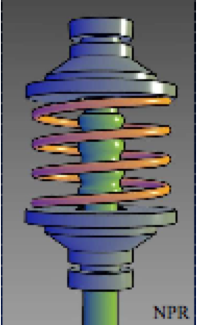
\includegraphics[height=0.25\textheight]{figs/nprcao.png}
\hspace{0.1cm}
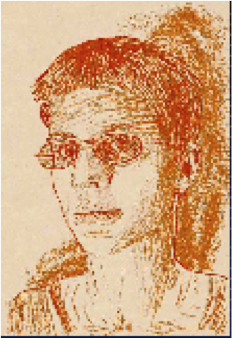
\includegraphics[height=0.25\textheight]{figs/npr-points.png}
\hspace{0.1cm}
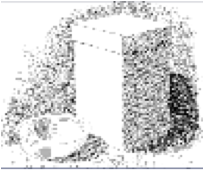
\includegraphics[height=0.25\textheight]{figs/npr-points2.png}
\end{center}

\end{frame}


\begin{frame}{Problématique}
\begin{itemize}
\item Associer à chaque pixel une intensité lumineuse qui dépend de :
\begin{itemize}
\item Des objets de la scène et de leurs propriétés physiques
\item Des sources lumineuses éclairant la scène
\item De la position des objets dans la scène
\item De la caméra virtuelle qui filme la scène
\begin{itemize}
\item position, orientation
\item caractéristiques techniques
\end{itemize}
\end{itemize}
\end{itemize}
\end{frame}

\begin{frame}{Le processus de rendu}
\begin{center}
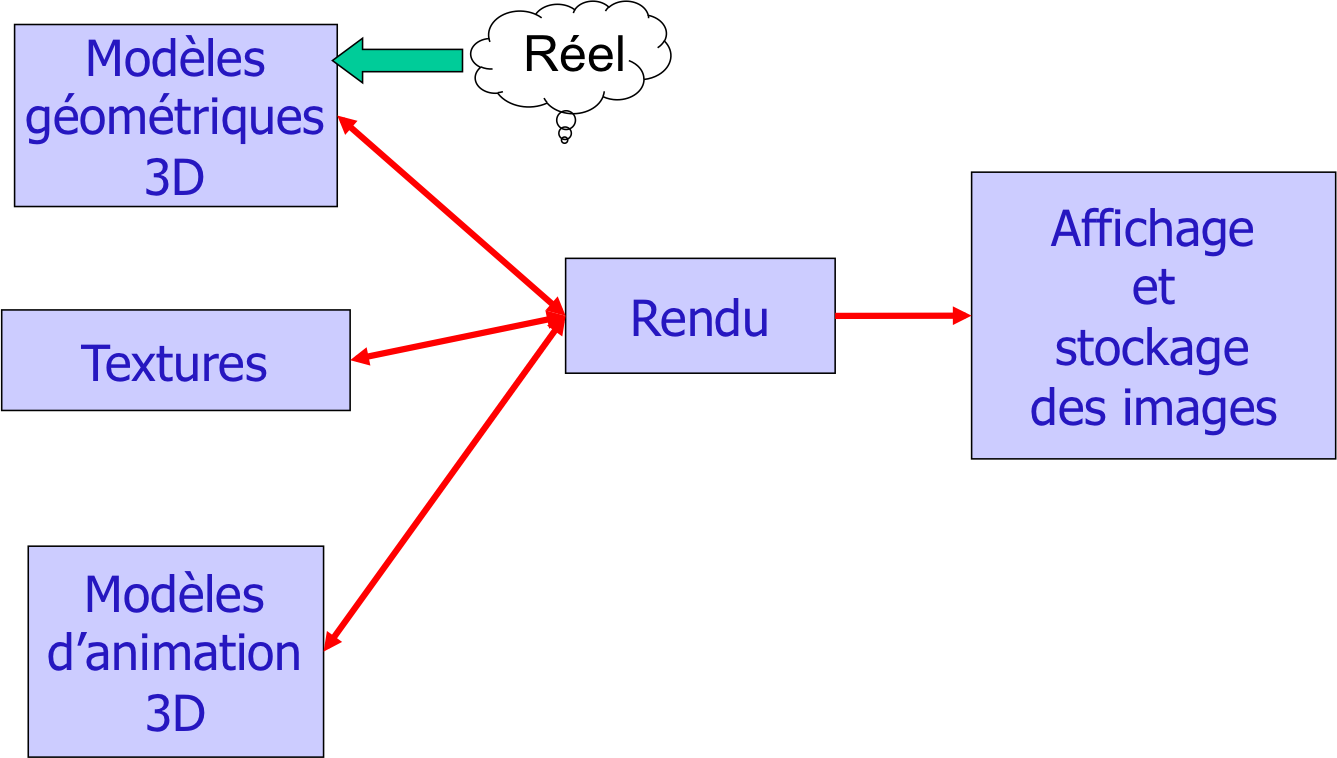
\includegraphics[height=.8\textheight]{figs/rendu.png}
\end{center}
\end{frame}

\begin{frame}{Rendu temps-réel}
\begin{center}
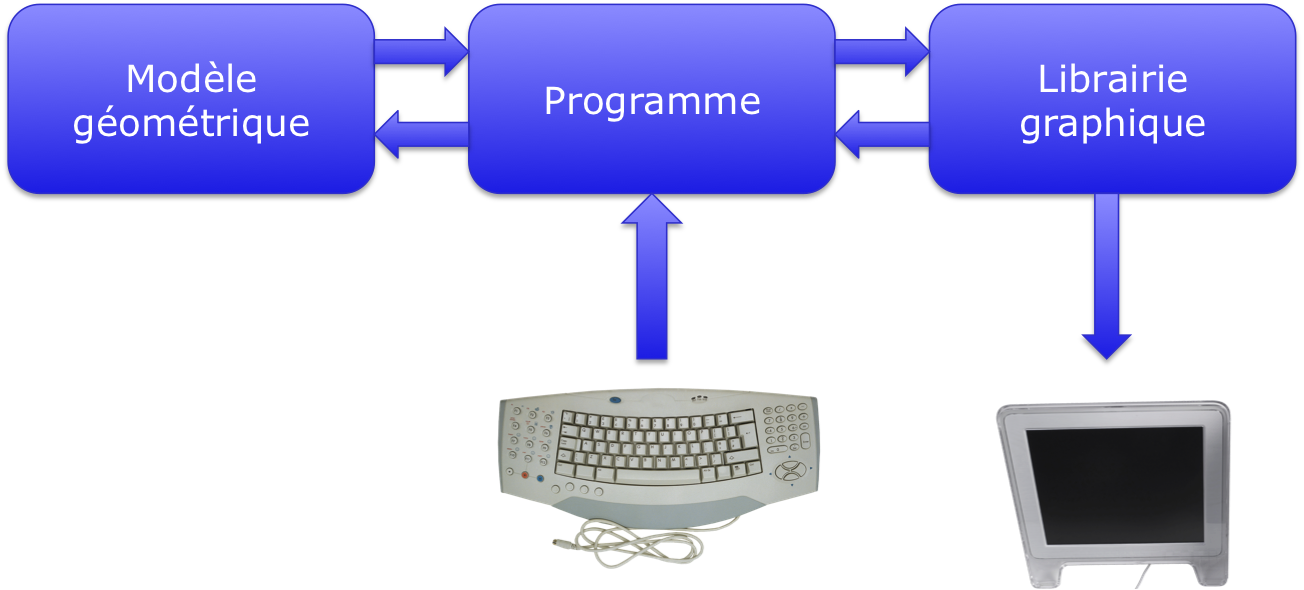
\includegraphics[width=.9\textwidth]{figs/rendurt.png}
\end{center}
\end{frame}

\begin{frame}{Modélisation géométrique}
\begin{center}
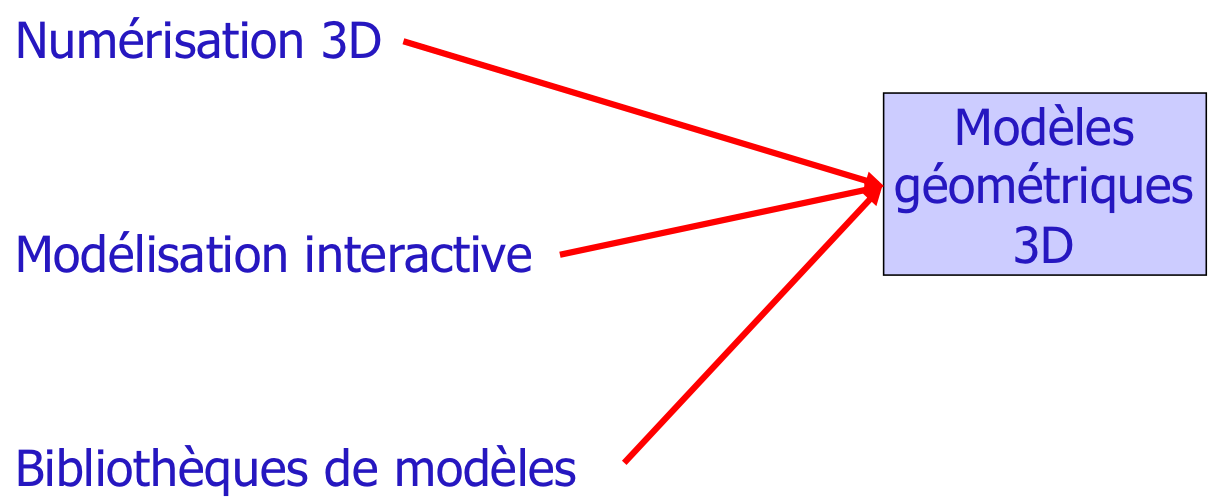
\includegraphics[width=.9\textwidth]{figs/modgeom.png}
\end{center}

\end{frame}

\begin{frame}{Animation}
\begin{center}
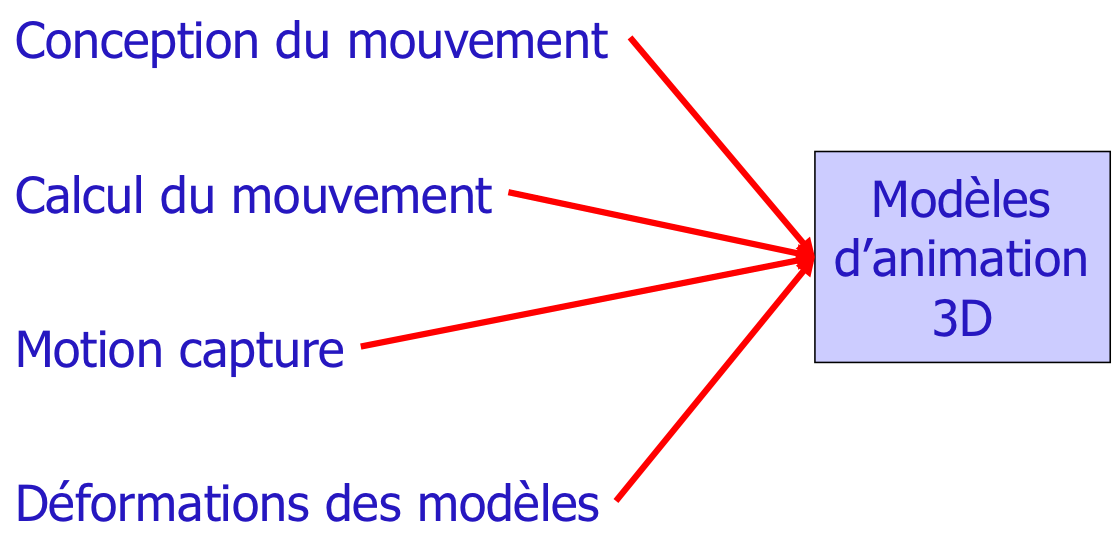
\includegraphics[width=.9\textwidth]{figs/anim.png}
\end{center}

\end{frame}

\begin{frame}{Modèles géométriques}
\begin{center}
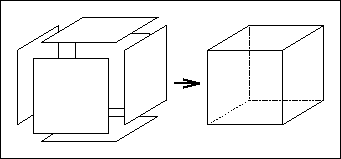
\includegraphics[height=1.8cm]{figs/brep.png}
\end{center}
\begin{itemize}
\item Description des objets
\begin{itemize}
\item Forme
\item Attributs
\item Comportements, propriétés
\end{itemize}
\item Stocké en mémoire par l'application, modifiable par l'application
\item Principe B-Rep (Boundary representation) : un solide est représenté par sa frontière extérieure
\item Plusieurs types de modèles (voir cours GEOMOD3D)
\begin{itemize}
\item Primitives (boites, cônes, sphères)
\item Surfaces triangulées
\item Surfaces de révolution
\item Combinaison de primitives
\end{itemize}
\end{itemize}
\end{frame}

\begin{frame}{Surfaces triangulées}
\begin{columns}
\begin{column}{.6\textwidth}
\begin{itemize}
\item Ensemble de triangles obtenus par
\begin{itemize}
\item construction
\item \textit{tessellation}
\end{itemize}
\item Normale au triangle
\begin{itemize}
\item définit l'intérieur/extérieur
\item Souvent implicite
\end{itemize}
\end{itemize}
\end{column}
\begin{column}{.39\textwidth}
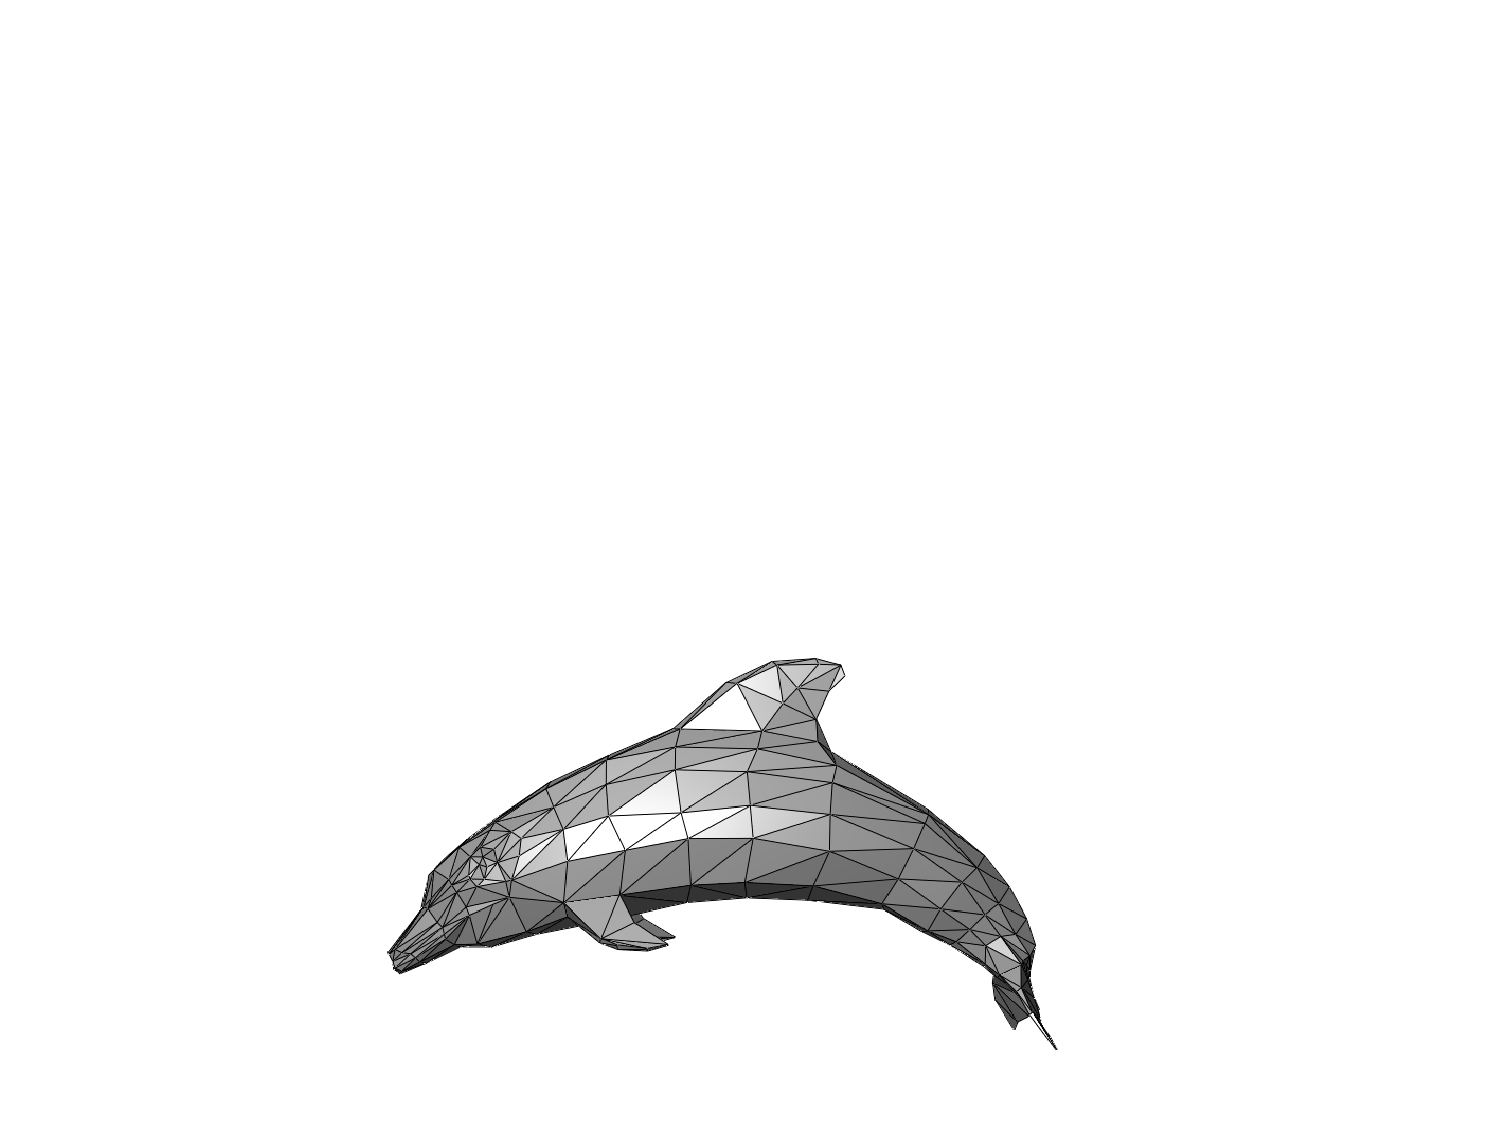
\includegraphics[width=\textwidth]{figs/dauphin.pdf}
\end{column}
\end{columns}
\end{frame}

\begin{frame}{Quelle quantité de triangles ?}
\begin{center}
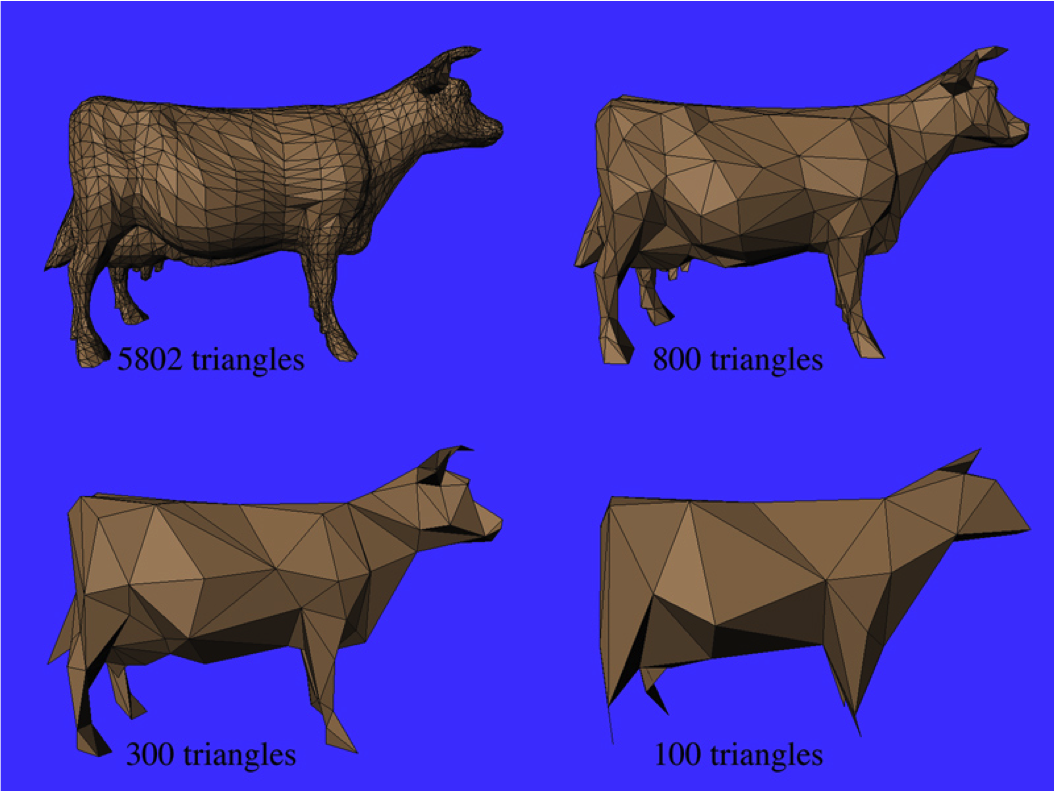
\includegraphics[height=.8\textheight]{figs/triangles}
\end{center}
\end{frame}

\begin{frame}{Surfaces de révolution}
\begin{columns}
\begin{column}{.6\textwidth}
\begin{itemize}
\item Un axe et un profil
\item L'objet peut être décomposé en facettes quadrangulaires
\item Et donc en triangles
\end{itemize}
\end{column}
\begin{column}{.39\textwidth}
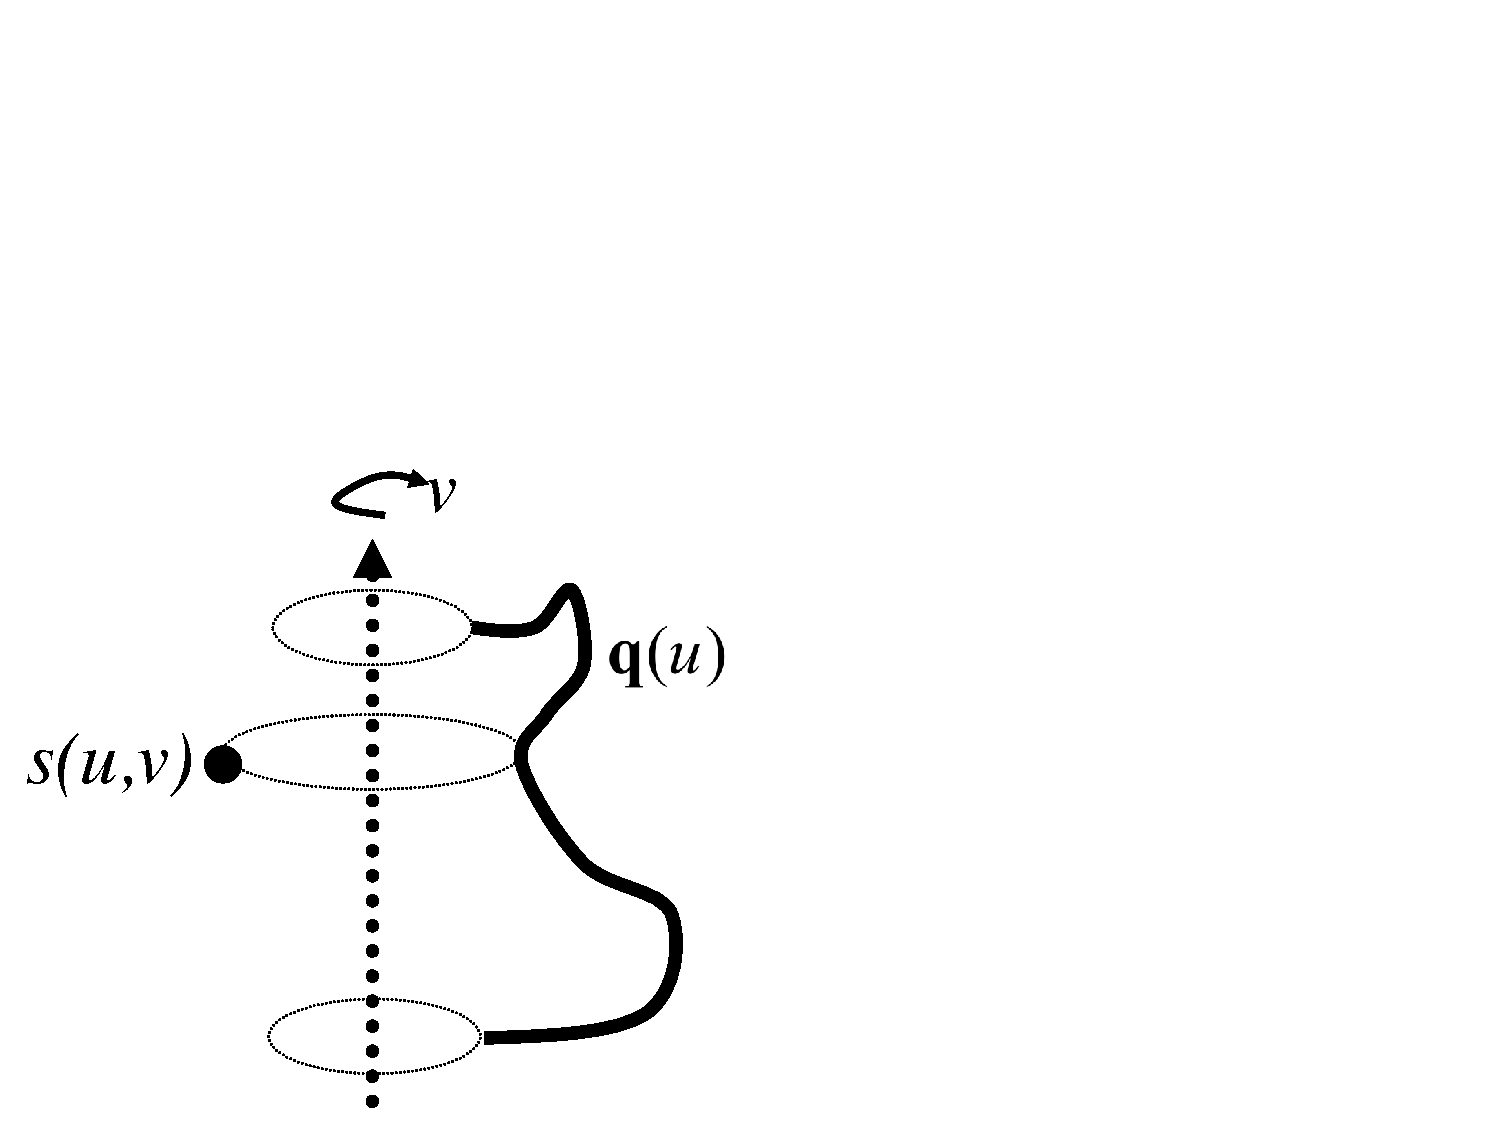
\includegraphics[height=.4\textheight]{figs/rev2.pdf} \\
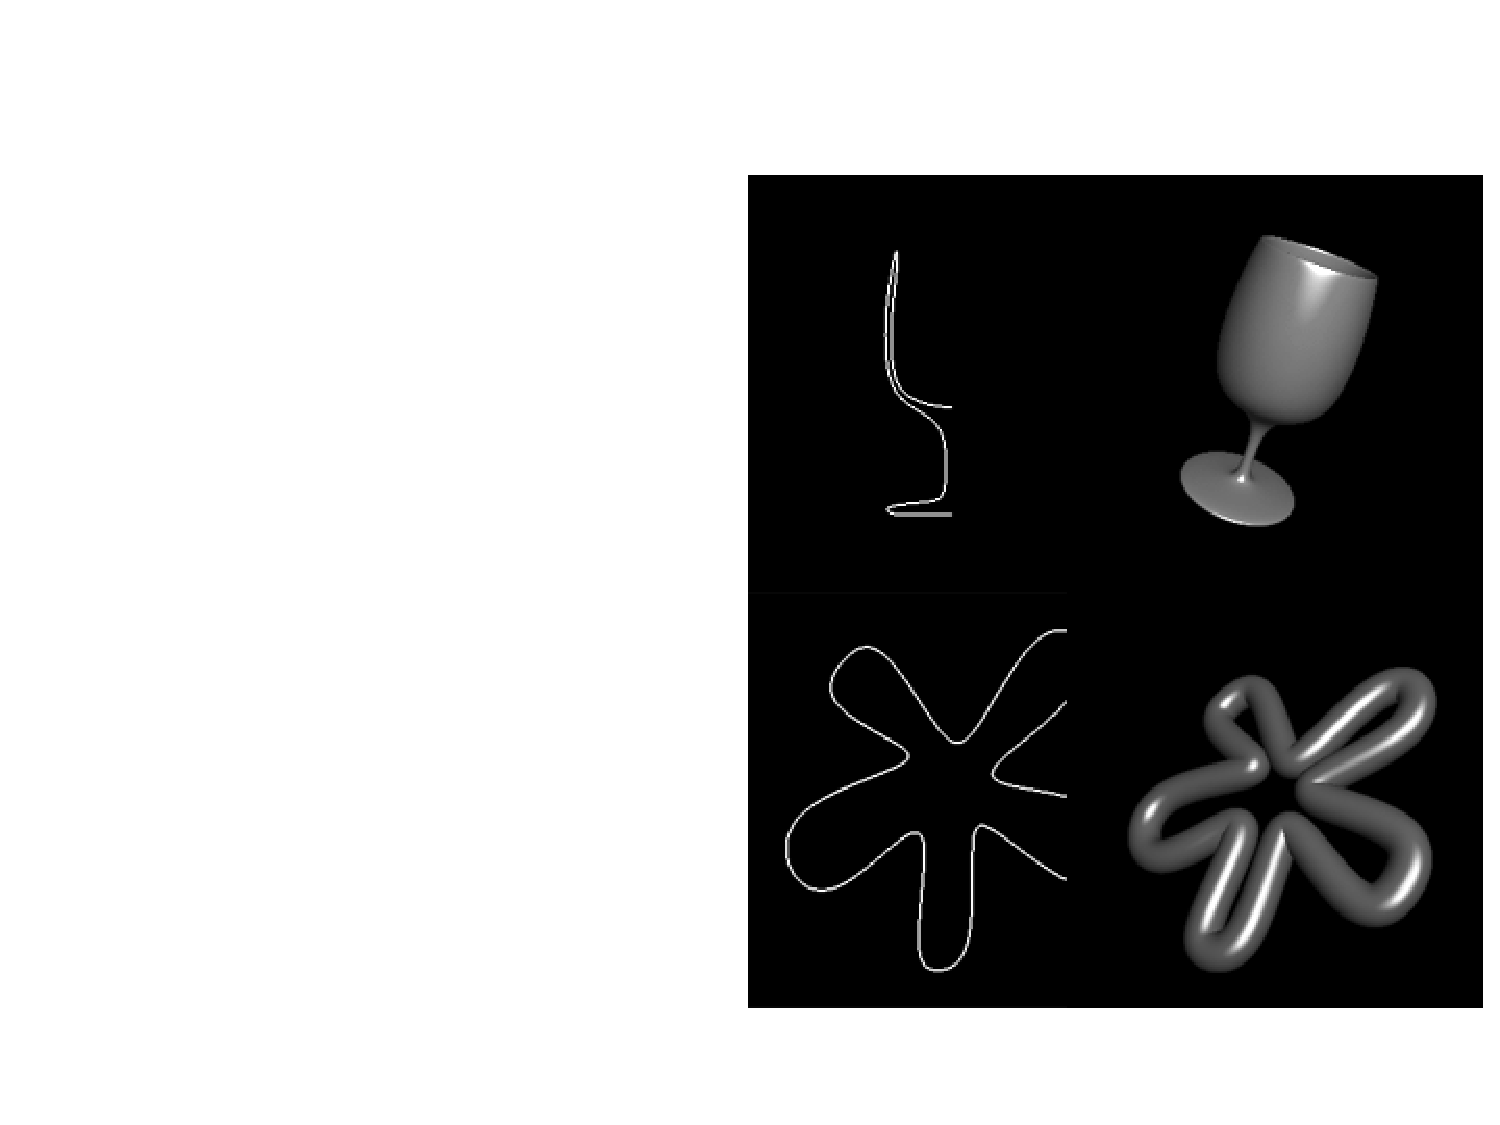
\includegraphics[height=.4\textheight]{figs/rev1.pdf}
\end{column}
\end{columns}
\end{frame}

\begin{frame}{CSG: constructive solid geometry}
\begin{columns}
\begin{column}{.6\textwidth}
\begin{itemize}
\item Combinaison de primitives géométriques
\item Opérateurs ensemblistes
\begin{itemize}
\item Union
\item Intersection
\item Différence
\end{itemize}
\item Très utilisé en CAO
\item Transformable (difficilement) en maillage triangulé
\item Utilisable directement dans certains algorithmes de rendu
\end{itemize}
\end{column}
\begin{column}{.39\textwidth}
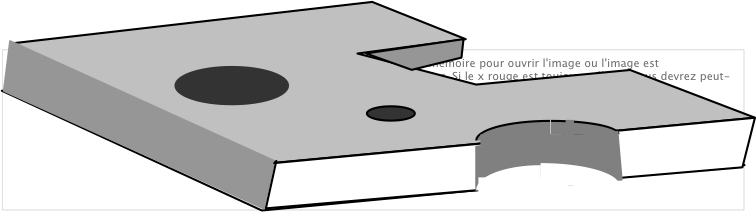
\includegraphics[width=.8\textwidth]{figs/csg1.png} \\
\vspace{1cm}
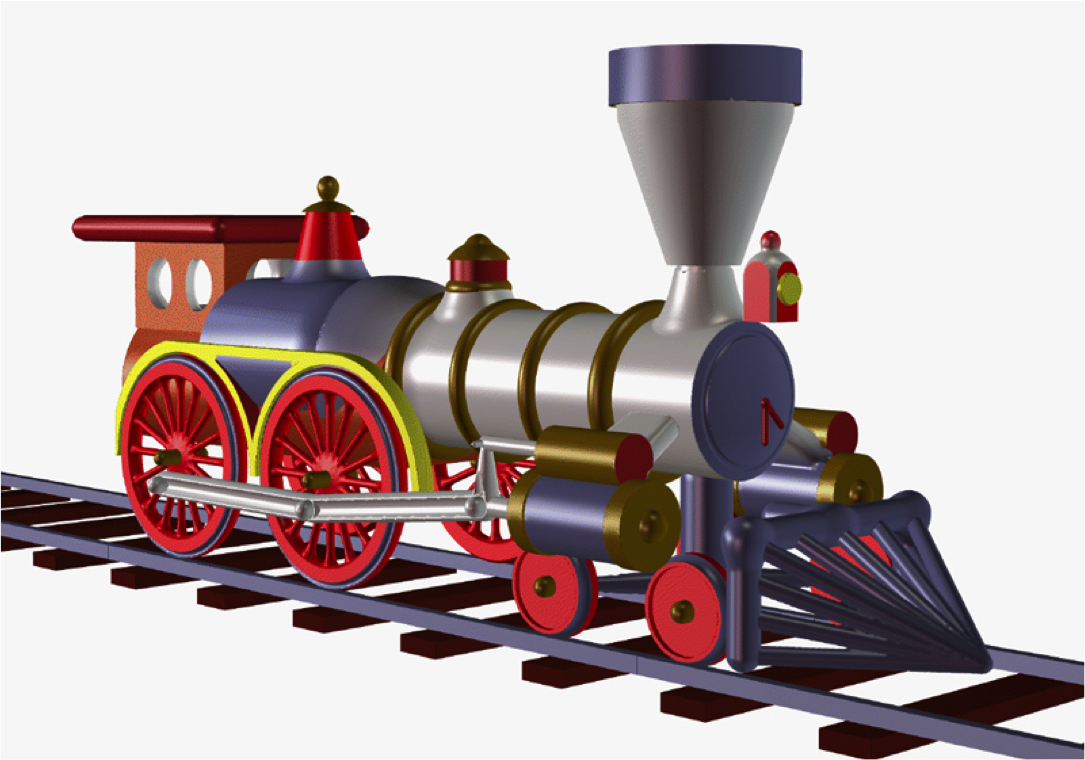
\includegraphics[width=.8\textwidth]{figs/csg2.png}
\end{column}
\end{columns}
\end{frame}

\subsection{Le pipeline graphique}

\begin{frame}{Pipeline graphique}
\begin{itemize}
\item Pipeline graphique : série de transformations géométriques
\end{itemize}
\begin{center}
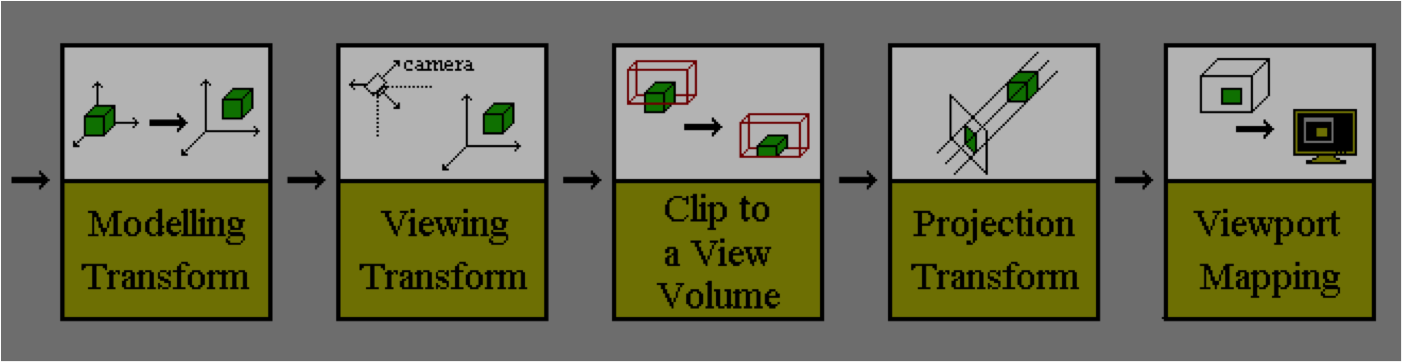
\includegraphics[width=.8\textwidth]{figs/pipeline.png}
\end{center}
\end{frame}

\begin{frame}{Exemple : série de transformations géométriques}
\begin{columns}
\begin{column}{.6\textwidth}
\begin{itemize}
\item<1-3> Objet dans son repère local
\item<2-3> Plusieurs objets
\item<3> Plusieurs objets vus de la caméra
\end{itemize}
\end{column}
\begin{column}{.39\textwidth}
\includegraphics<1>[width=.8\textwidth]{figs/pp1.png}
\includegraphics<2>[width=.8\textwidth]{figs/pp2.png}
\includegraphics<3>[width=.8\textwidth]{figs/pp3.png}

\end{column}
\end{columns}
\end{frame}

\begin{frame}{Types de repère}
\begin{itemize}
\item Repère objet (plusieurs)
\item Repère observateur
\item Repère écran
\begin{itemize}
\item Entre l'observateur et la scène
\end{itemize}
\end{itemize}
\begin{center}
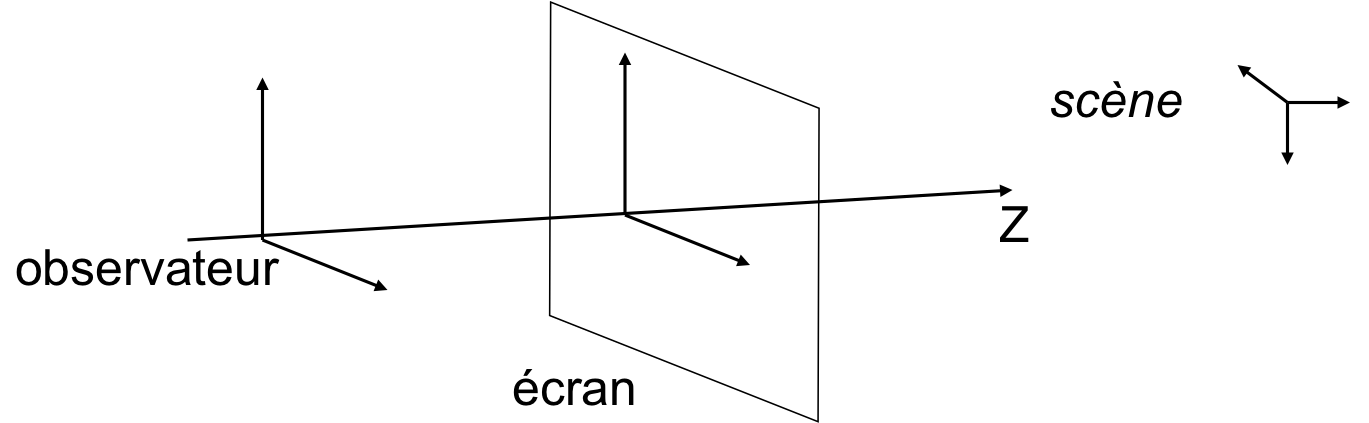
\includegraphics[width=.8\textwidth]{figs/reperes.png}
\end{center}
\end{frame}

\begin{frame}{Modèles hiérarchiques}
\begin{itemize}
\item Les triangles (ainsi que les autres modèles vus précédemment) sont les blocs servant à construire des objets réels plus complexes
\item Les modèles hiérarchiques servent à créer des objets du monde réel par agrégation de formes primitives en des objets plus complexes
\end{itemize}
\begin{center}
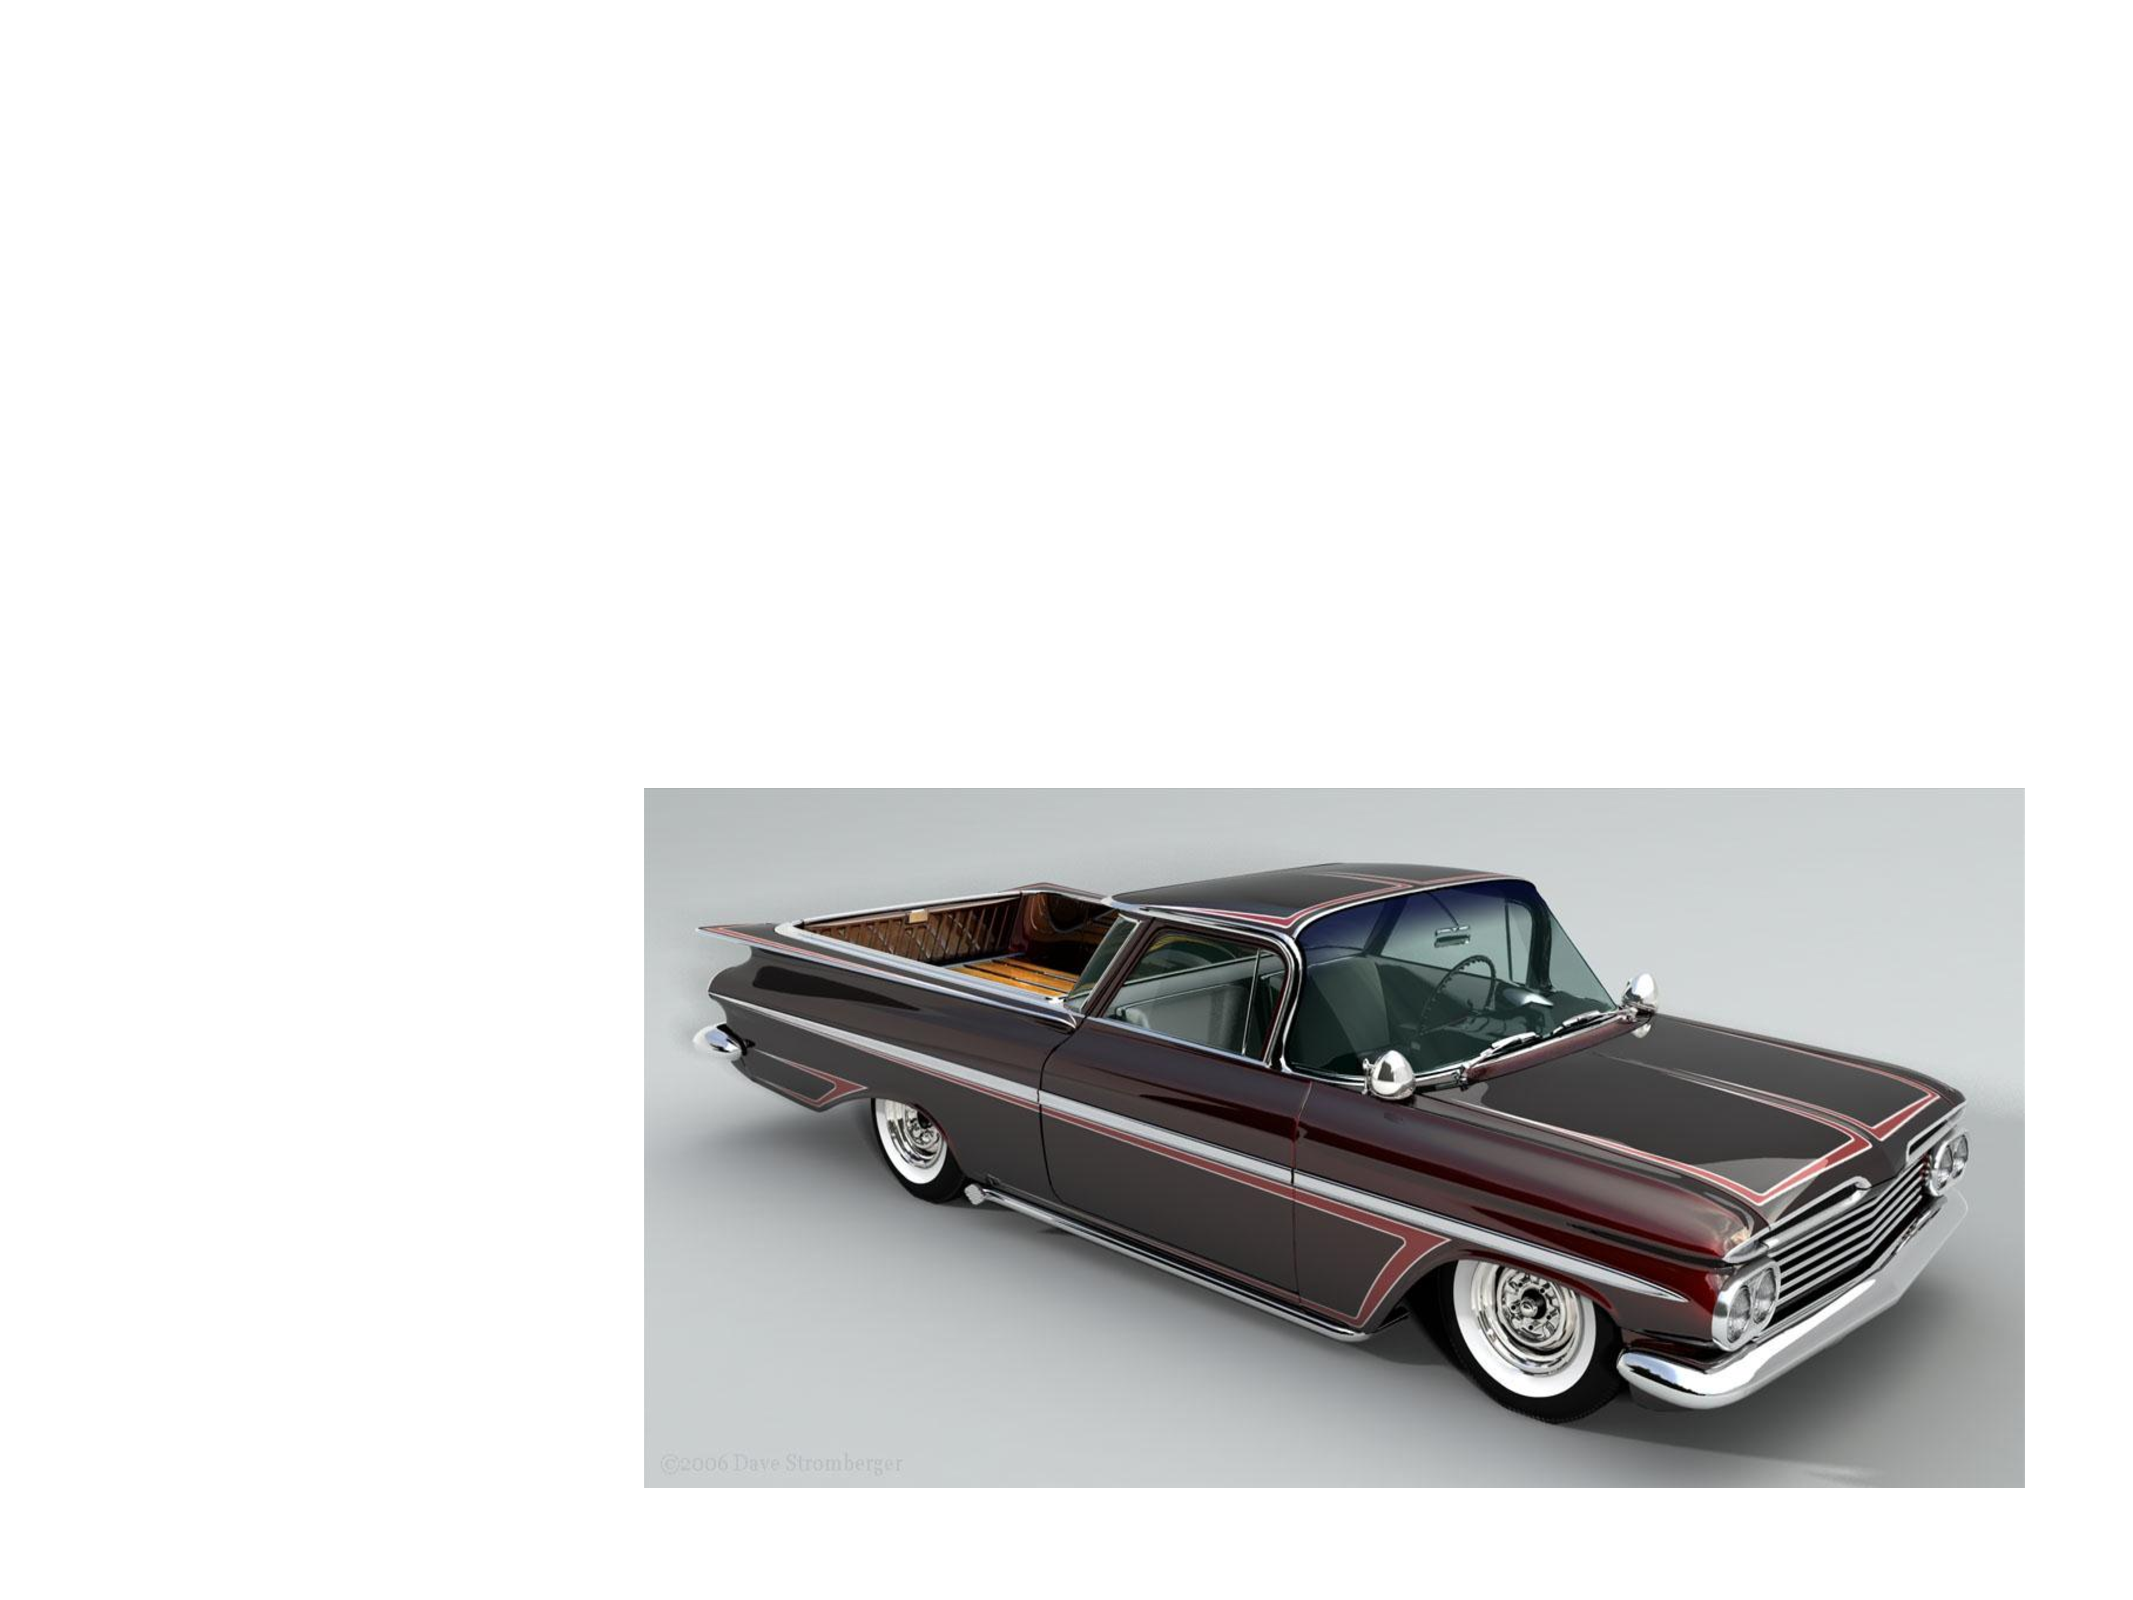
\includegraphics[height=.4\textheight]{figs/car.pdf}
\end{center}

\end{frame}

\begin{frame}{Hiérarchie d'un modèle}
\begin{center}
\includegraphics<1>[height=.8\textheight]{figs/piece1.pdf}
\includegraphics<2>[height=.8\textheight]{figs/piece2.pdf}
\includegraphics<3>[height=.8\textheight]{figs/piece3.pdf}
\includegraphics<4>[height=.8\textheight]{figs/piece4.pdf}
\includegraphics<5>[height=.8\textheight]{figs/piece5.pdf}
\includegraphics<6>[height=.8\textheight]{figs/piece6.pdf}
\end{center}
\end{frame}

\begin{frame}{Vers une notion de <<graphe de scène>>}
\begin{center}
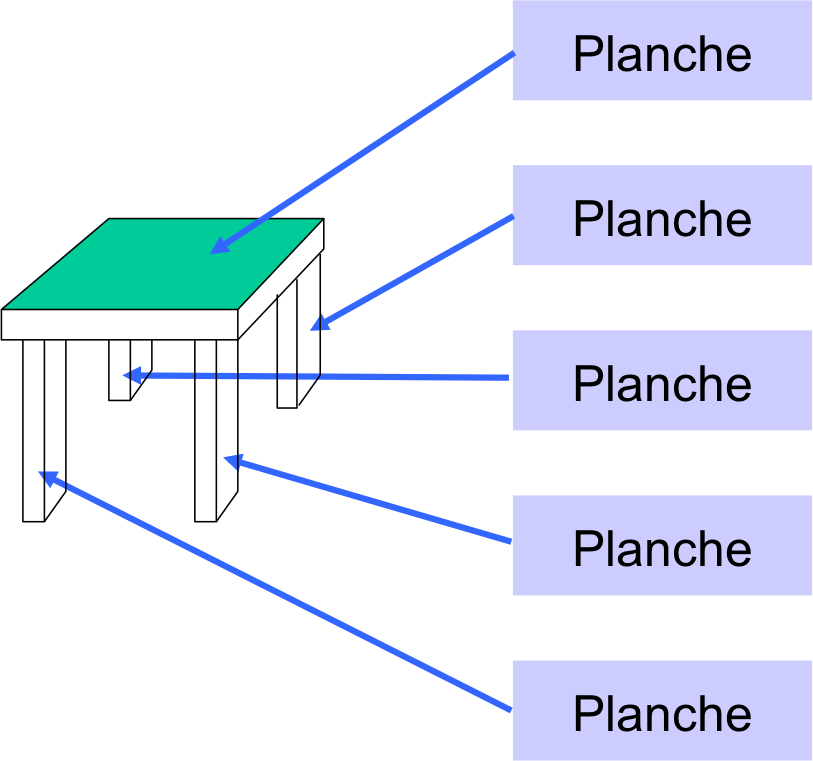
\includegraphics[height=.8\textheight]{figs/table.png}
\end{center}
\end{frame}

\begin{frame}{Vers une notion de <<graphe de scène>>}
\begin{center}
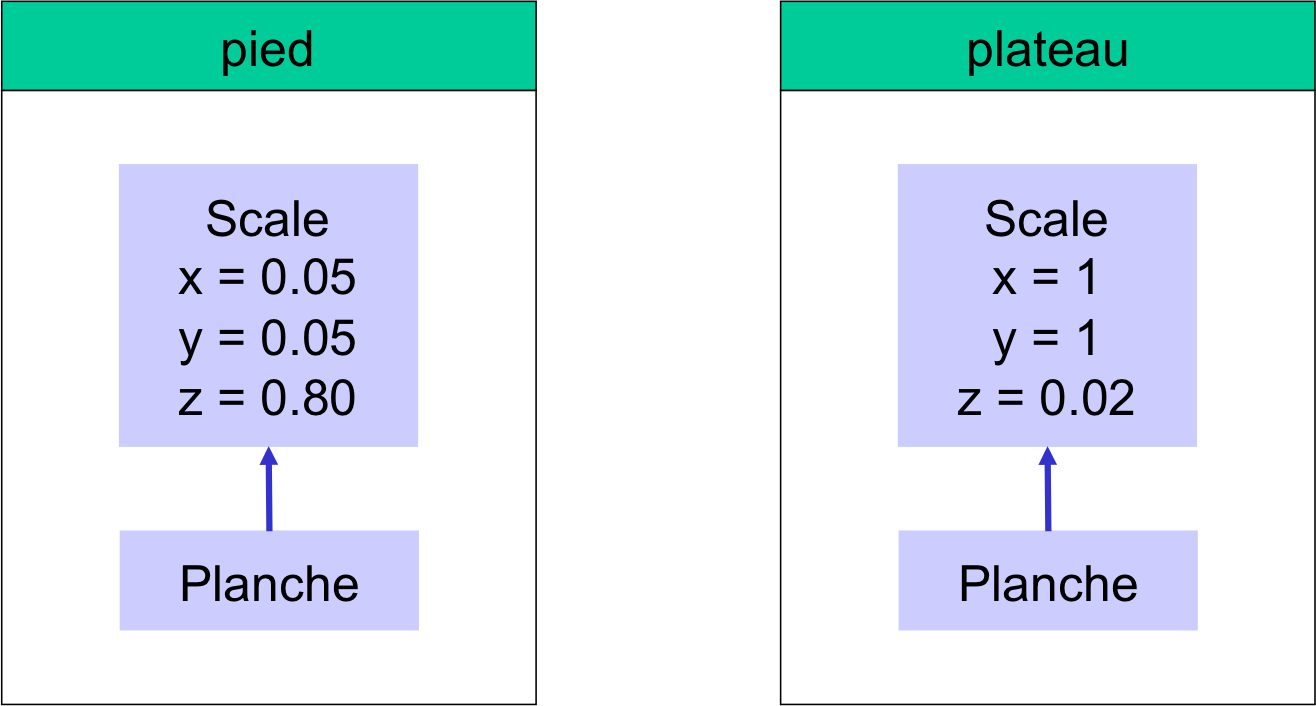
\includegraphics[height=.6\textheight]{figs/table2.png}
\end{center}
\end{frame}

\begin{frame}{Vers une notion de <<graphe de scène>>}
\begin{center}
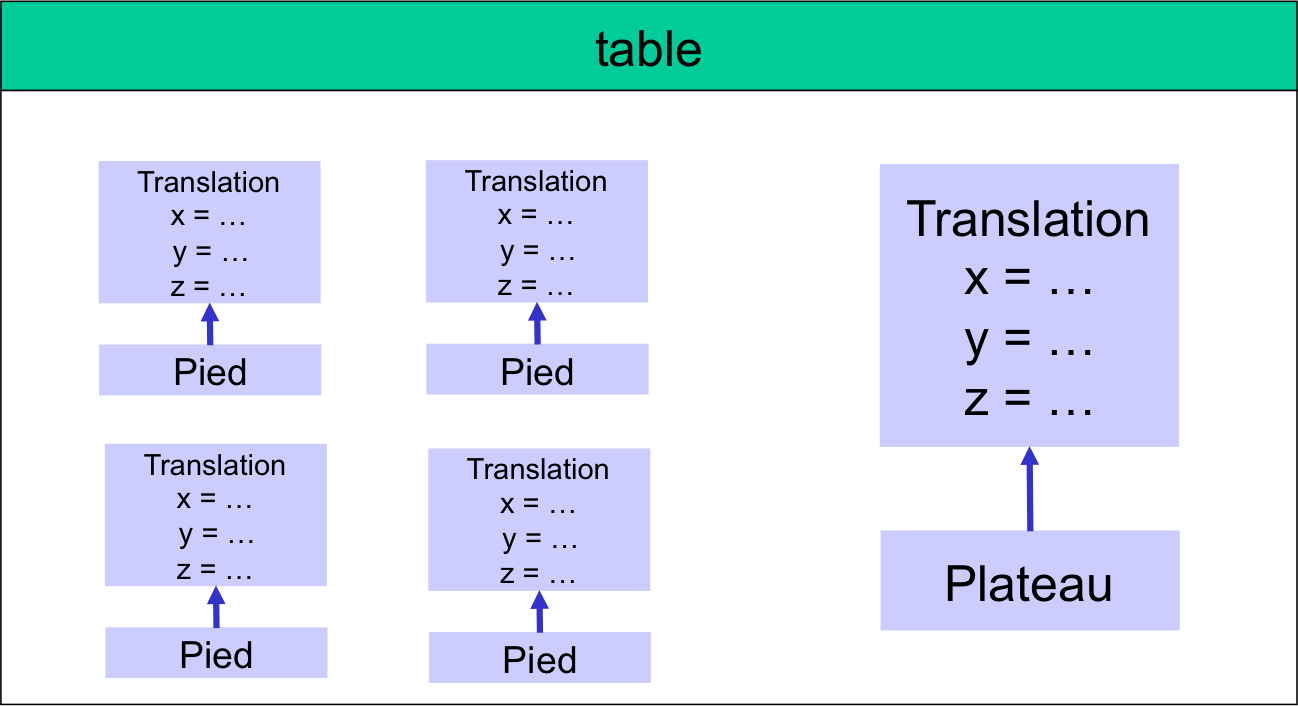
\includegraphics[height=.6\textheight]{figs/table3.png}
\end{center}
\end{frame}

\begin{frame}{Vers une notion de <<graphe de scène>>}
\begin{center}
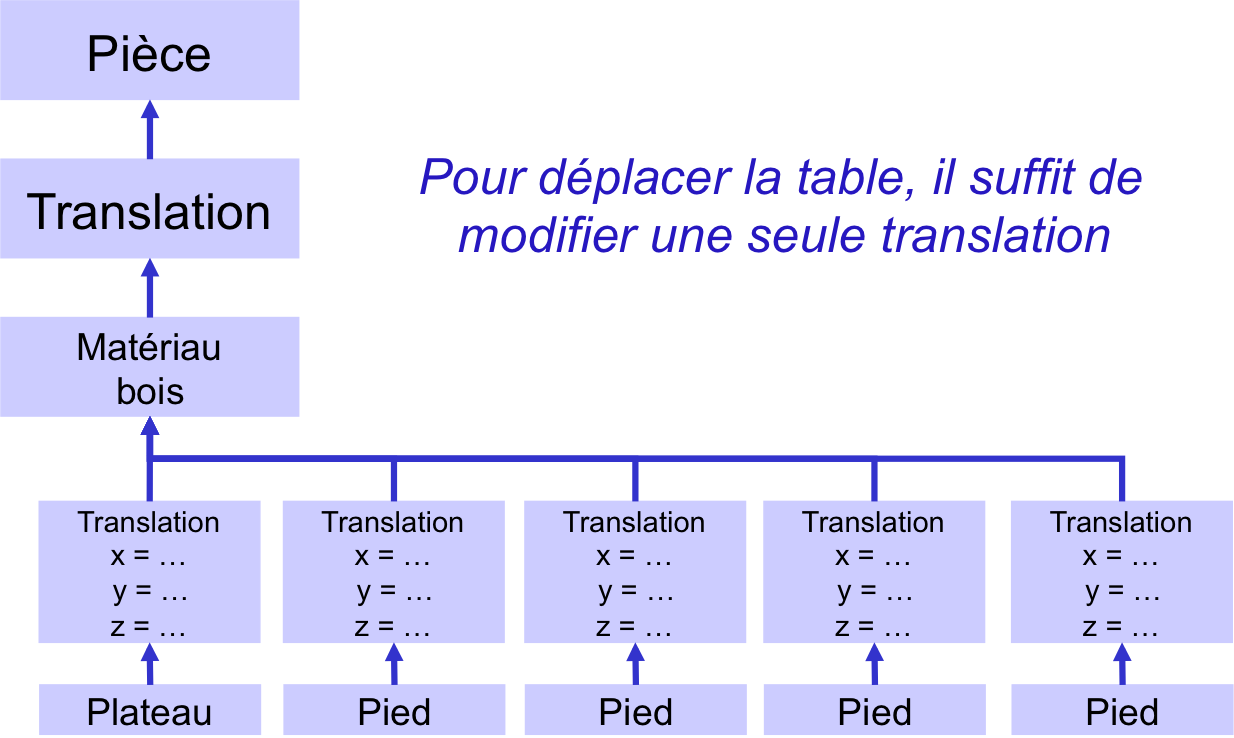
\includegraphics[height=.6\textheight]{figs/table4.png}
\end{center}
\end{frame}

\begin{frame}{Différentes formes de graphes de scène}
\begin{center}
\includegraphics<1>[height=.8\textheight]{figs/sg1.png}
\includegraphics<2>[height=.8\textheight]{figs/sg2.png}
\includegraphics<3>[height=.5\textheight]{figs/sg3.png}
\includegraphics<4>[height=.6\textheight]{figs/sg4.png}
\end{center}
\end{frame}


\begin{frame}{Graphe de scène}
\begin{columns}
\begin{column}{.6\textwidth}
\begin{itemize}
\item Structure de données pratique pour la représentation de scènes
\begin{itemize}
\item Géométrie (dont maillages)
\item Transformations géométriques
\item Matériaux, couleurs
\item Multi-instanciations
\end{itemize}
\item Basé sur un simple arbre hiérarchique
\item Utile pour l'animation et la manipulation
\begin{itemize}
\item Exemple : figure articulée
\end{itemize}
\item Utile pour le rendu
\begin{itemize}
\item Accélération du lancer de rayons
\item Gestion des occlusions
\end{itemize}
\end{itemize}
\end{column}
\begin{column}{.39\textwidth}
\begin{center}
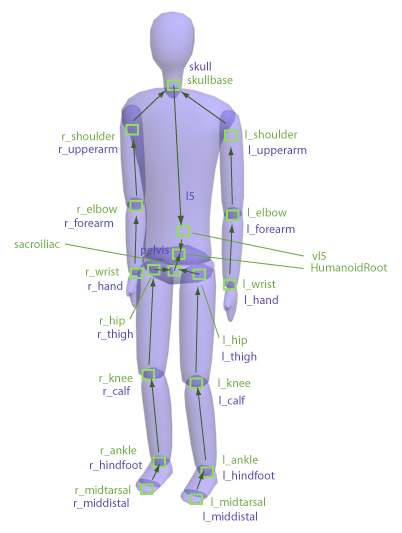
\includegraphics[width=.8\textwidth]{figs/hanim.jpg}
\end{center}
\end{column}
\end{columns}
\end{frame}

\begin{frame}{Modèles hiérarchiques et OpenGL}
\begin{alertblock}{Remarque}
Ou pourquoi il faut éviter de programmer des choses complexes avec OpenGL
\end{alertblock}
\begin{itemize}
\item OpenGL s'apparente à de la programmation procédurale
\begin{itemize}
\item Séquence de dessin des différentes primitives de l'objet
\item Des opérations qui modifient la transformation courante
\begin{itemize}
\item \texttt{glTranslate()}, \texttt{glScale()}...
\end{itemize}
\end{itemize}
\item Les transformations géométriques affectent l'état courant, et donc tout ce qui suit
\item En OpenGL, on va utiliser \texttt{glPushMatrix()} et \texttt{glPopMatrix()} pour enregistrer / récupérer l'état courant
\item Lorsqu'on rencontre un noeud \textit{Transform}
\begin{itemize}
\item \texttt{glPushMatrix()}
\item Application de la transformation géométrique
\item dessin du noeud et de ses sous-noeuds
\item \texttt{glPopMatrix()}
\end{itemize}
\end{itemize}
\end{frame}


\subsection{Coordonnées homogènes}

\begin{frame}{En deux dimensions}
\begin{itemize}
\item 2D : plus facile à représenter mais exactement le même principe
\item Transformation géométrique d'un point $\mathbf{X}=(x,y)$
\begin{eqnarray*}
x' & = & f(x,y) \\
y' & = & g(x,y)
\end{eqnarray*}
\item Comment peut-on représenter les transformations courantes ?
\end{itemize}
\end{frame}

\begin{frame}{Translation}
\begin{columns}
\begin{column}{.6\textwidth}
\begin{itemize}
\item Très simple
\begin{eqnarray*}
x' & = & x + t_x \\
y' & = & y + t_y
\end{eqnarray*}
\item Notation vectorielle
\end{itemize}
\begin{eqnarray}
\mathbf{X'} & = & \mathbf{X} + \mathbf{t}
\end{eqnarray}
\end{column}
\begin{column}{.39\textwidth}
\begin{center}
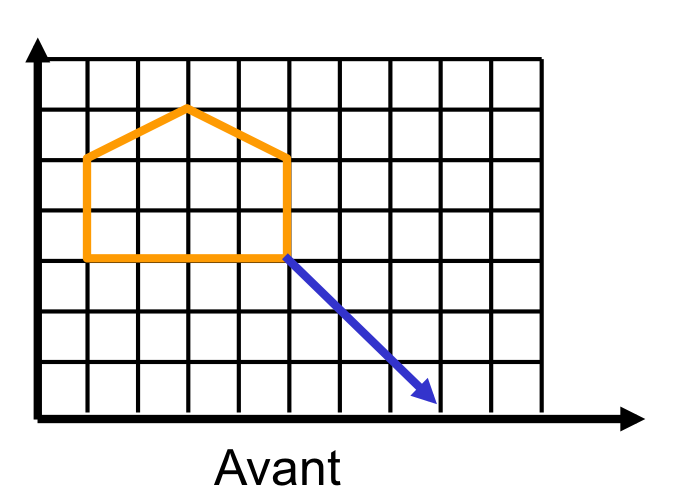
\includegraphics[width=.7\textwidth]{figs/trans2d1.png} \\
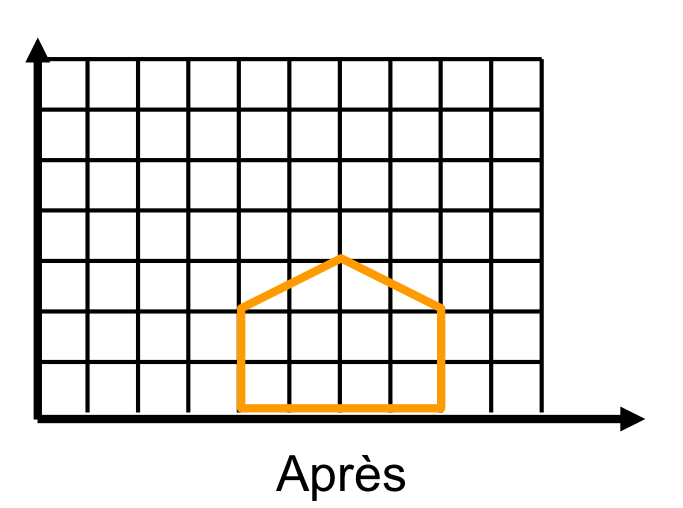
\includegraphics[width=.7\textwidth]{figs/trans2d2.png} \\

\end{center}
\end{column}
\end{columns}
\end{frame}

\begin{frame}{Changement d'échelle}
\begin{columns}
\begin{column}{.6\textwidth}
\begin{itemize}
\item Centré sur l'origine
\item Il suffit d'appliquer une translation préalable
\begin{eqnarray*}
x' & = & x . s_x \\
y' & = & y . s_y
\end{eqnarray*}
\item Notation vectorielle
\end{itemize}
\begin{eqnarray*}
\mathbf{X'} & = & \mathbf{S}\mathbf{X} \\
\mathrm{avec}\  \mathbf{S} & = & \left(
\begin{array}{cc}
s_x & 0 \\
0 & s_y \\
\end{array}
\right)
\end{eqnarray*}
\end{column}
\begin{column}{.39\textwidth}
\begin{center}
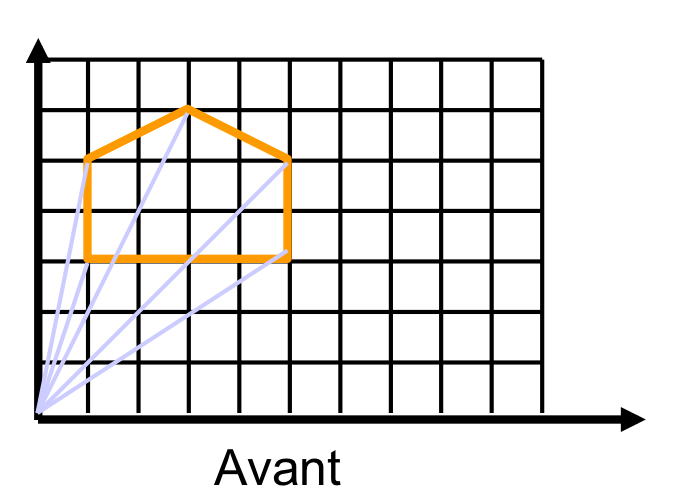
\includegraphics[width=.7\textwidth]{figs/scale1.png} \\
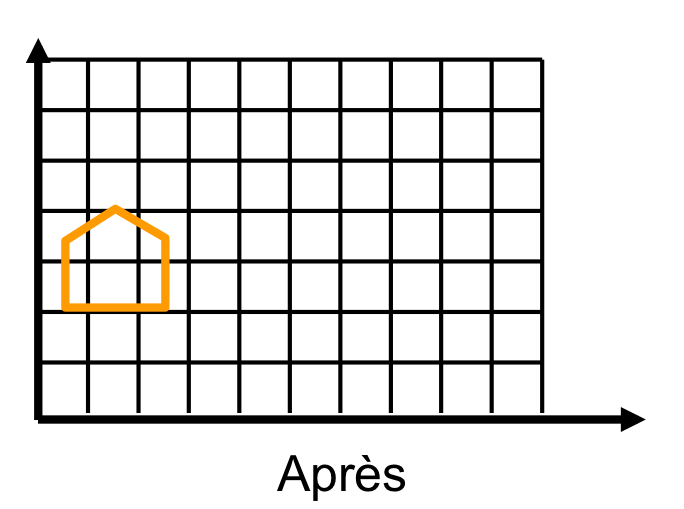
\includegraphics[width=.7\textwidth]{figs/scale2.png} \\

\end{center}
\end{column}
\end{columns}
\end{frame}

\begin{frame}{Rotation, notation unifiée}
\begin{itemize}
\item De façon similaire, on écrit la rotation d'un angle $\theta$ par rapport à l'origine :
\begin{eqnarray*}
\mathbf{X'} & = & \mathbf{R}\mathbf{X} \\
\mathrm{avec}\  \mathbf{R} & = & \left(
\begin{array}{cc}
\cos \theta & -\sin \theta \\
\sin \theta & \cos \theta \\
\end{array}
\right)
\end{eqnarray*}
\item On souhaiterait avoir une notation unifiée
\begin{itemize}
\item Pas un mélange d'additions et de rotations
\item Un seul type d'opérations : bien pour les cartes graphiques
\end{itemize}
\end{itemize}
\end{frame}

\begin{frame}{Coordonnées homogènes}
\begin{itemize}
\item Outil géométrique très puissant
\begin{itemize}
\item Utilisé partout en image (infographie, vision...)
\item Voir géométrie projective
\end{itemize}
\item Consiste à ajouter une $n+1$-ème coordonnée à tout point de dimension $n$
\item Par exemple, en 2D
$$ \mathbf{\overline{X}} = \left( \begin{array}{c} x \\ y \\ w
\end{array}\right), w \neq 0 $$
\item Deux points sont égaux ssi $x'/w'=x/w$ et $y'/w'=y/w$
\item $w=0$ utile pour représenter les points à l'infini (points de fuite, projections...)
\end{itemize}
\end{frame}

\begin{frame}{Translation en coordonnées homogènes}
\begin{center}
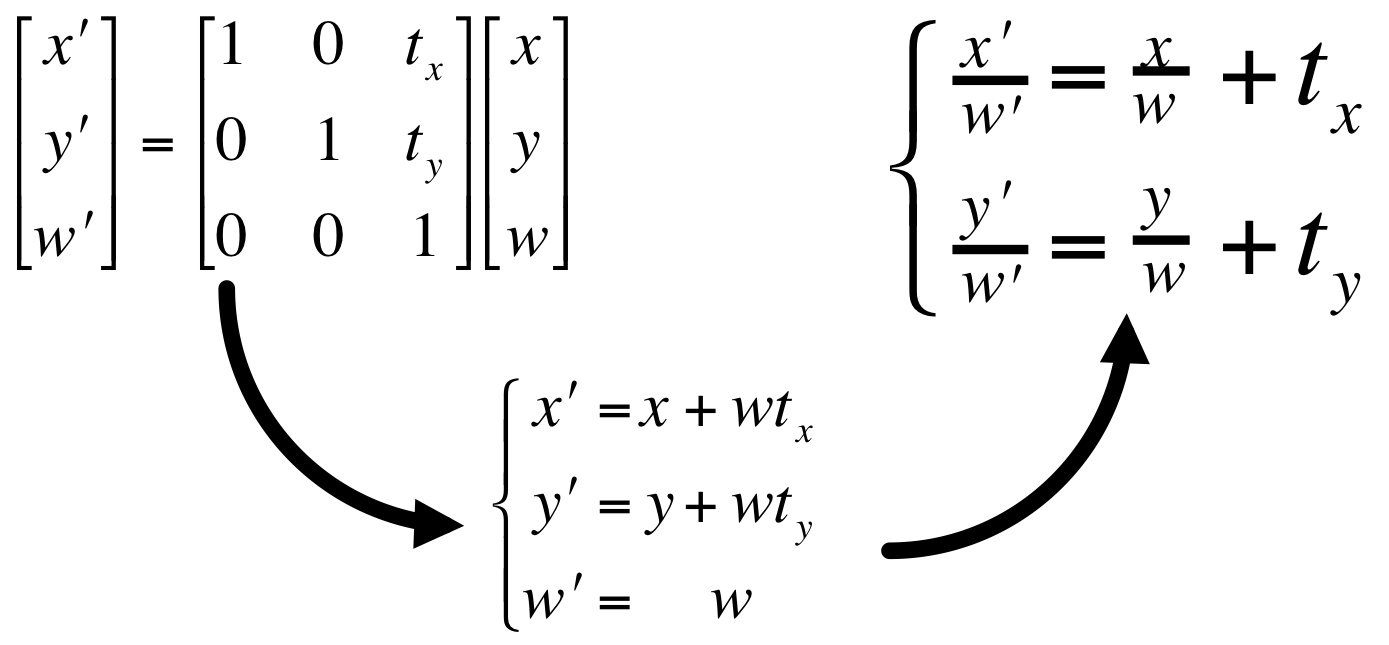
\includegraphics[width=.8\textwidth]{figs/transh.png}
\end{center}
\end{frame}

\begin{frame}{Changement d'échelle en coordonnées homogènes}
\begin{center}
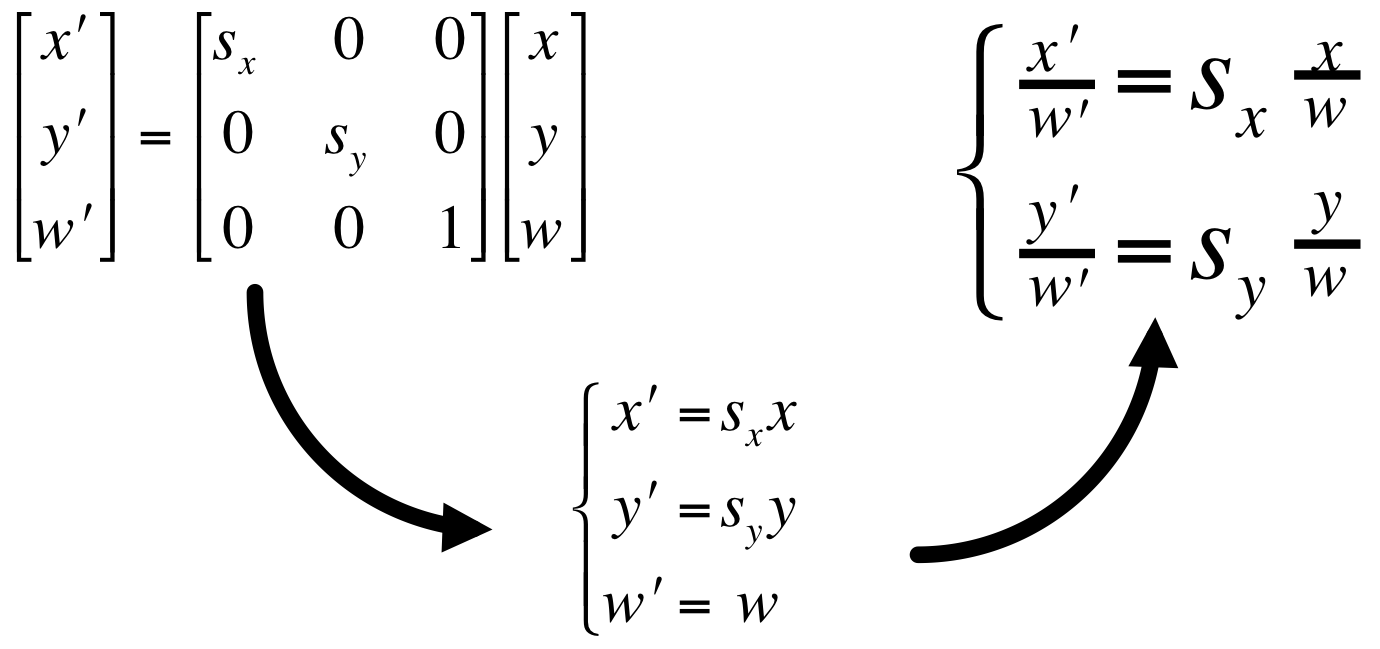
\includegraphics[width=.8\textwidth]{figs/scaleh.png}
\end{center}
\end{frame}

\begin{frame}{Rotation en coordonnées homogènes}
\begin{center}
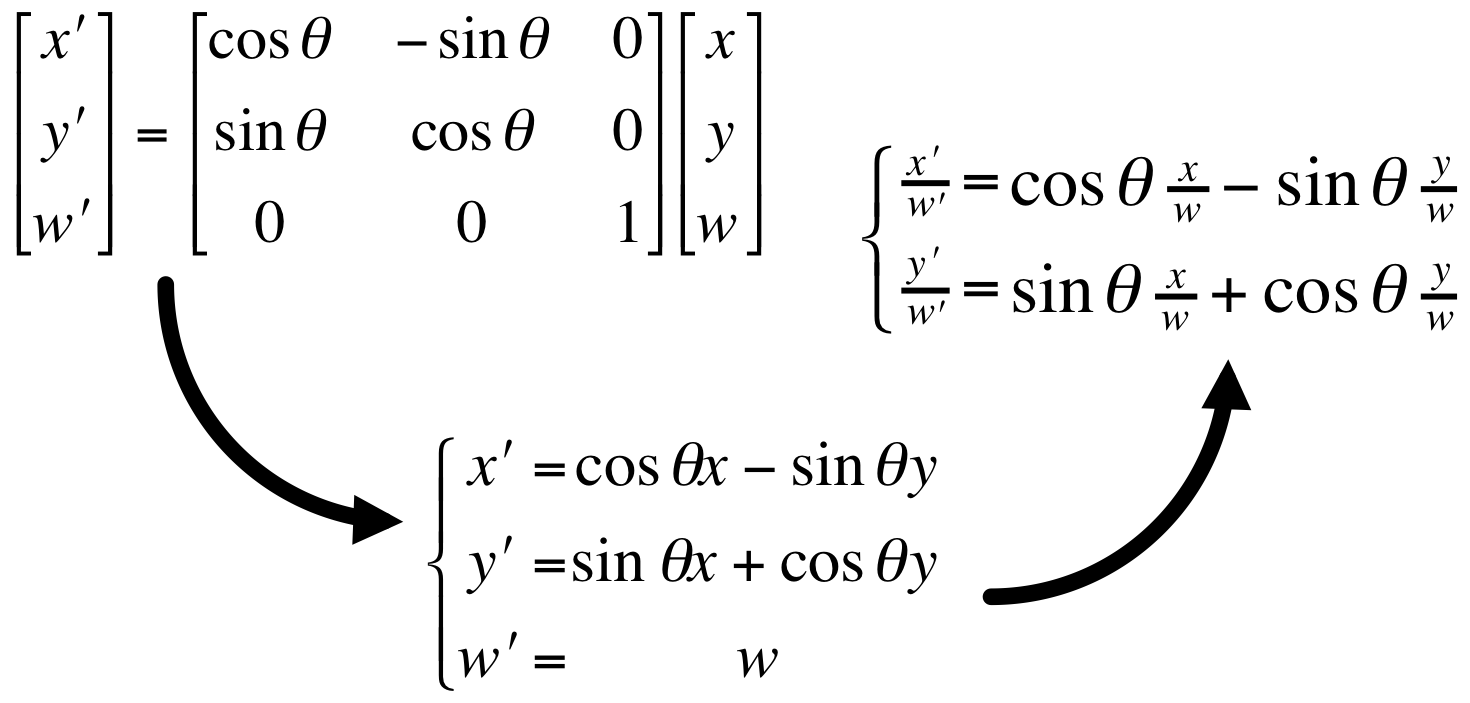
\includegraphics[width=.8\textwidth]{figs/roth.png}
\end{center}
\end{frame}

\begin{frame}{Composition de transformations}
\begin{itemize}
\item Toutes les transformations homogènes s'expriment sous forme de matrices
\item Il suffit de multiplier les matrices !
\item En se rappelant que la multiplication de matrices n'est pas commutative
\item Exemple : rotation autour d'un point $\mathbf{Q}$
\begin{itemize}
\item Translater $\mathbf{Q}$ à l'origine
\item Effectuer la rotation
\item Translater en retour vers $\mathbf{Q}$
$$
\mathbf{Q'} = -\mathbf{T_Q R_{\theta} T_Q P}
$$
\end{itemize}
\end{itemize}
\end{frame}


\begin{frame}{Translations en 3D}
\begin{center}
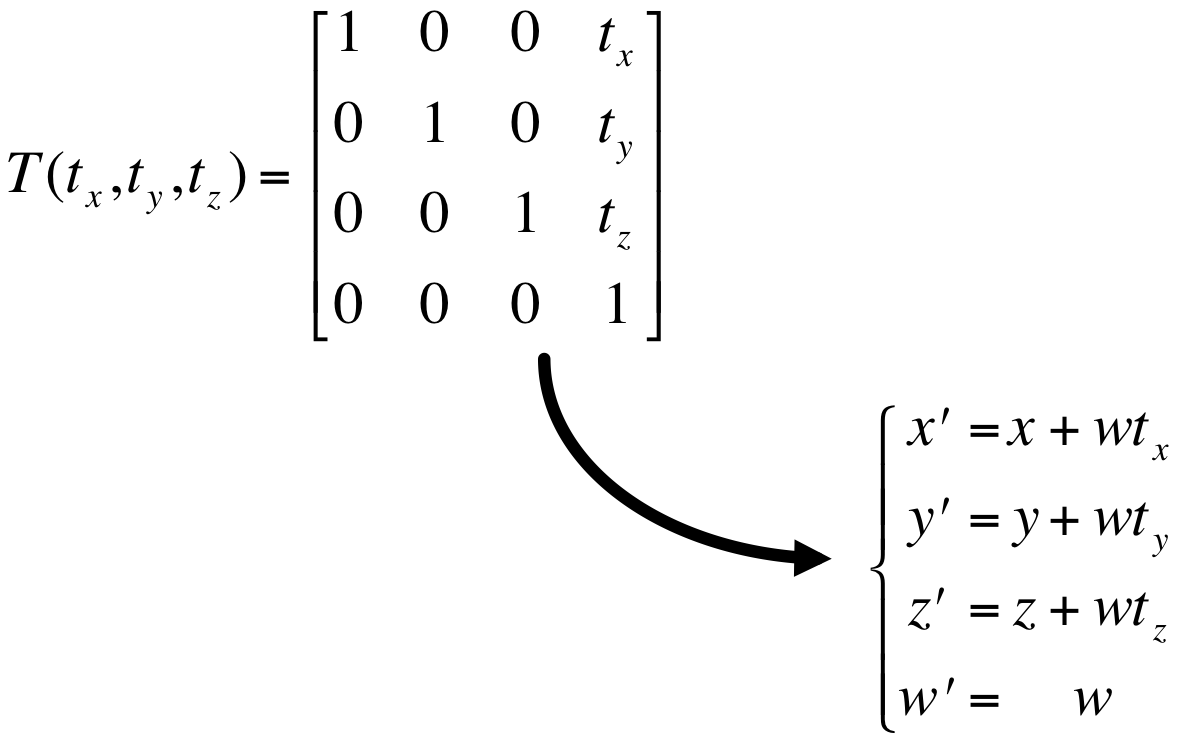
\includegraphics[width=.8\textwidth]{figs/transh3.png}
\end{center}
\end{frame}

\begin{frame}{Changements d'échelle en 3D}
\begin{center}
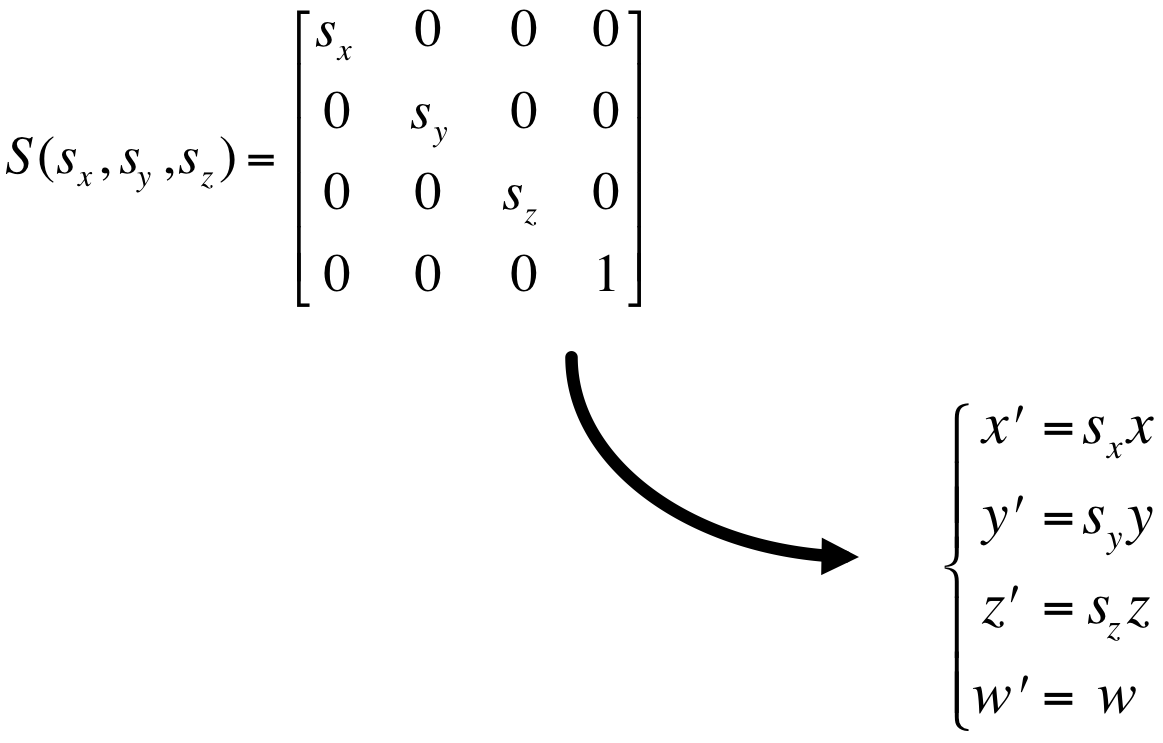
\includegraphics[width=.8\textwidth]{figs/scaleh3.png}
\end{center}
\end{frame}

\begin{frame}{Rotations en 3D}
\begin{itemize}
\item Rotation en 3D : définie par un axe et un angle
\item La matrice peut être construite à partir de l'axe et de l'angle
\item Expression directe avec un peu de calcul vectoriel
\begin{itemize}
\item Outil pratique : les quaternions
\end{itemize}
\item OpenGL peut le faire pour vous
\begin{itemize}
\item \texttt{glRotatef(angle,x,y,z)}
\end{itemize}
\end{itemize}
\end{frame}

\begin{frame}{Bilan : transformations 3D}
\begin{itemize}
\item Toutes les transformations 3D s'expriment sous forme de matrice homogène
\begin{itemize}
\item translations, rotations, changement d'échelle
\item et même d'autres que nous verrons plus tard
\end{itemize}
\item et donc leur combinaison comme une multiplication de matrices homogènes
\item La bibliothèque graphique fournit les fonctions adéquates
\begin{itemize}
\item \texttt{glTranslatef(x,y,z)}
\item \texttt{glRotatef(angle,x,y,z)}
\item \texttt{glScalef(x,y,z)}
\end{itemize}
\end{itemize}
\end{frame}

\begin{frame}{Composition de transformations avec OpenGL}
\begin{itemize}
\item Outils pour construire ses transformations
\begin{itemize}
\item \texttt{glLoadIdentity()}
\item \texttt{glLoadMatrixf()}
\item \texttt{glMultMatrixf()}
\end{itemize}
\item Gestion de la hiérarchie
\begin{itemize}
\item \texttt{glPushMatrix()}
\item \texttt{glPopMatrix()}
\end{itemize}
\item Mais aussi des fonctions de plus haut niveau !
\begin{itemize}
\item \texttt{gluLookAt(Eyex, Eyey, Eyez,Centerx, Centery, Centerz, upx, upy, upz)}
\item \texttt{gluPerspective( fovy, aspect, zNear, zFar )}
\end{itemize}
\end{itemize}
\end{frame}

\subsection{Projections}

\begin{frame}{Caméra virtuelle}
\begin{center}
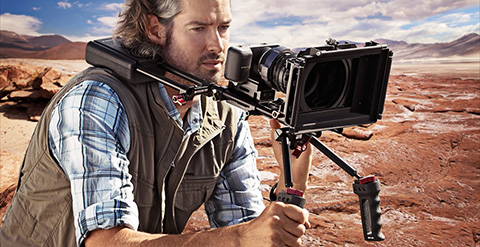
\includegraphics[width=3cm]{figs/camerar.jpg}
\end{center}
\begin{itemize}
\item Métaphore de la caméra
\begin{itemize}
\item Définir une caméra virtuelle qui va filmer la scène (virtuelle)
\item Restitution sur un moniteur 2D
\end{itemize}
\item Il faut
\begin{itemize}
\item Définir les caractéristiques de la caméra
\item Placer et orienter la caméra
\item Prendre les images et les afficher
\end{itemize}
\end{itemize}
\end{frame}

\begin{frame}{Différentes projections}
\begin{center}
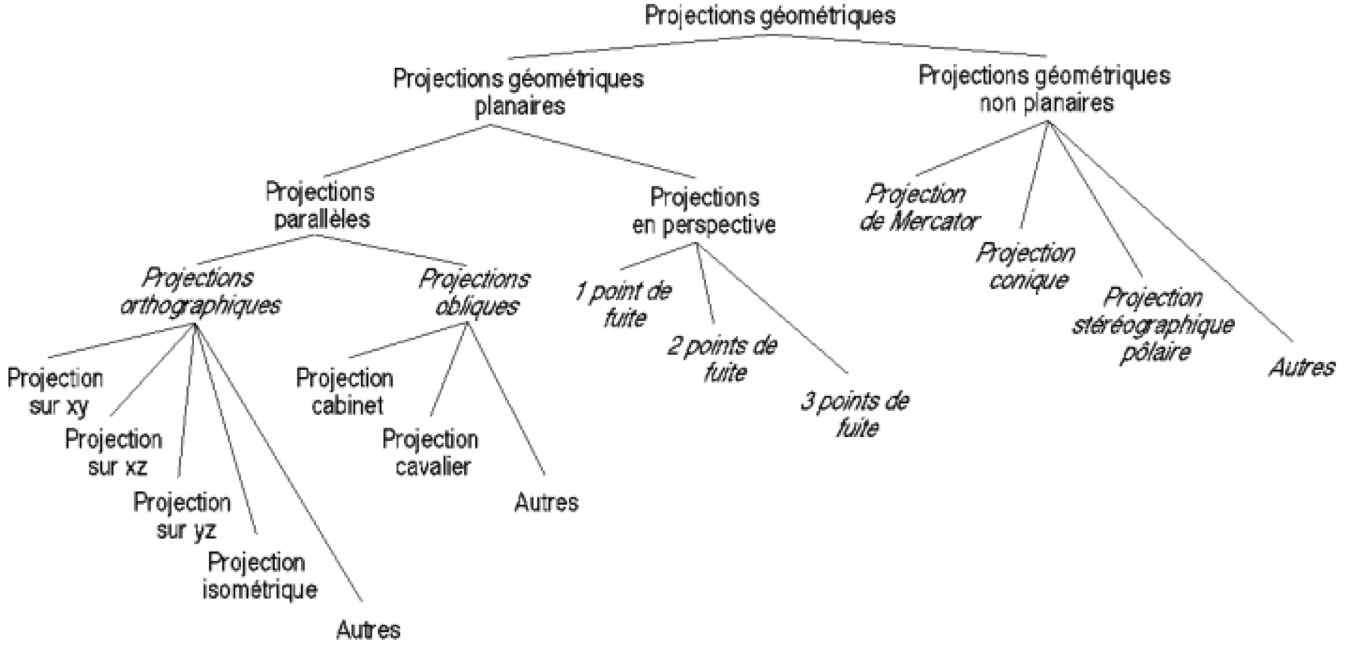
\includegraphics[width=.8\textwidth]{figs/projections.png}
\end{center}
\end{frame}

\begin{frame}{Quelle projection ?}
\begin{center}
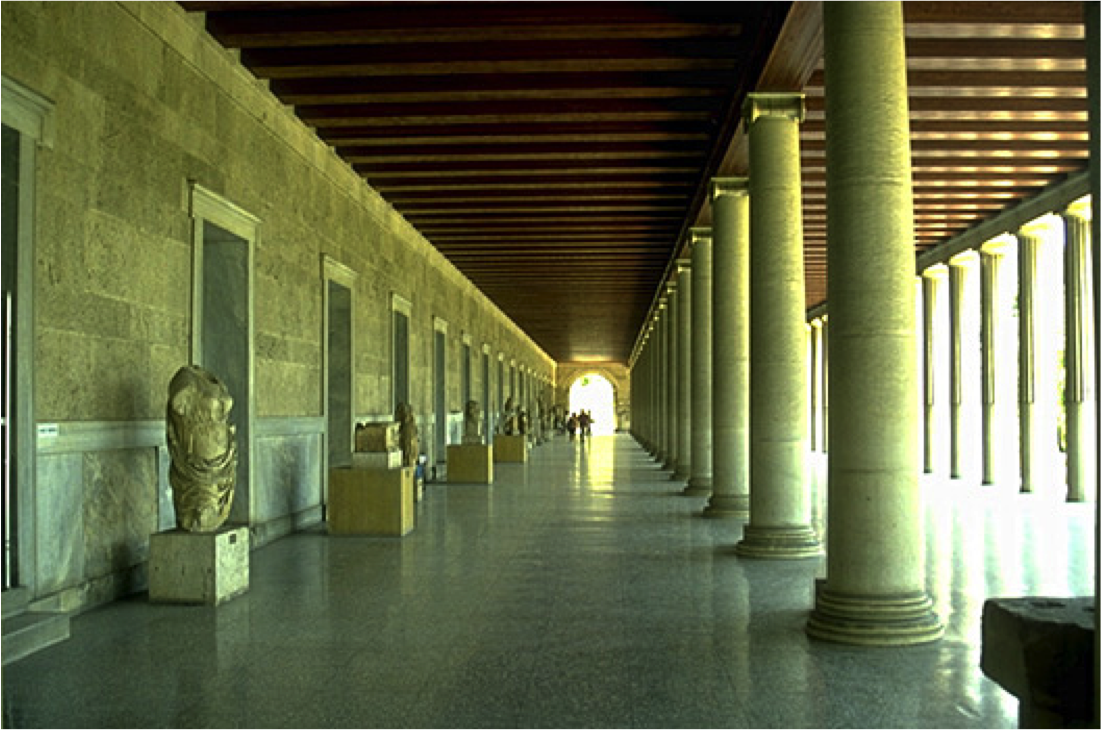
\includegraphics[width=.8\textwidth]{figs/athenes.png}
\end{center}
\end{frame}

\begin{frame}{Projection parallèle vs. perspective}
\begin{center}
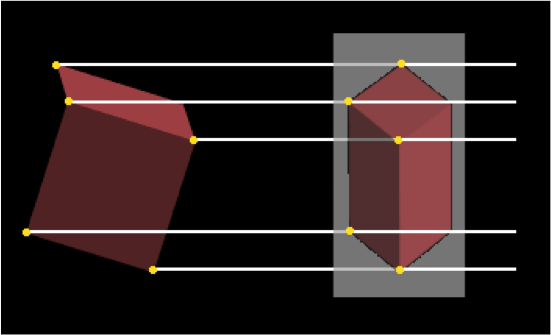
\includegraphics[height=3.7cm]{figs/projpar.png} \\
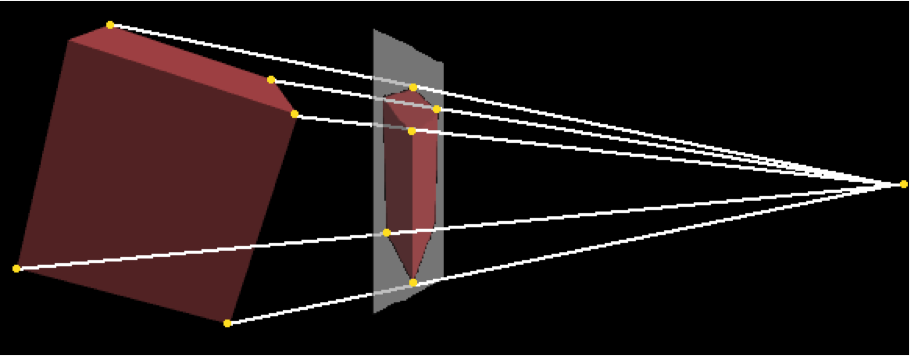
\includegraphics[height=3.7cm]{figs/projpersp.png} \\

\end{center}
\end{frame}

\begin{frame}{Projection parallèle vs. perspective : résultat}
\begin{center}
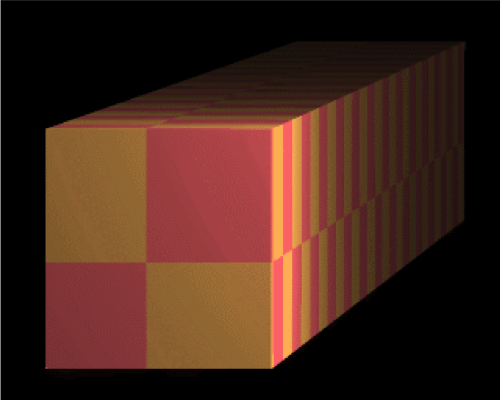
\includegraphics[height=3.7cm]{figs/projparr.png} \hspace{1cm}
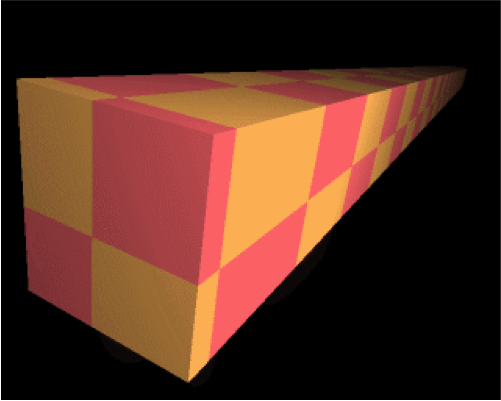
\includegraphics[height=3.7cm]{figs/projpersp1.png} \\

\end{center}
\begin{itemize}
\item L'\oe il humain utilise une projection centrale (perspective), tout comme une caméra
\end{itemize}
\end{frame}

\begin{frame}{Projection perspective simple}
\begin{center}
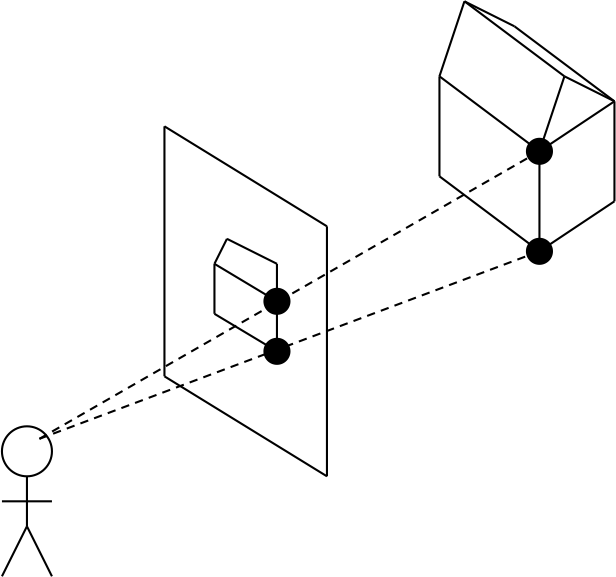
\includegraphics[height=.6\textheight]{figs/persp1.png}
\end{center}
\end{frame}

\begin{frame}{Projection perspective simple}
\begin{itemize}
\item Caméra dans l'axe des $z$
\item Point focal à l'origine
\item Plan image sur le plan XY à une distance $f$
\end{itemize}
\begin{center}
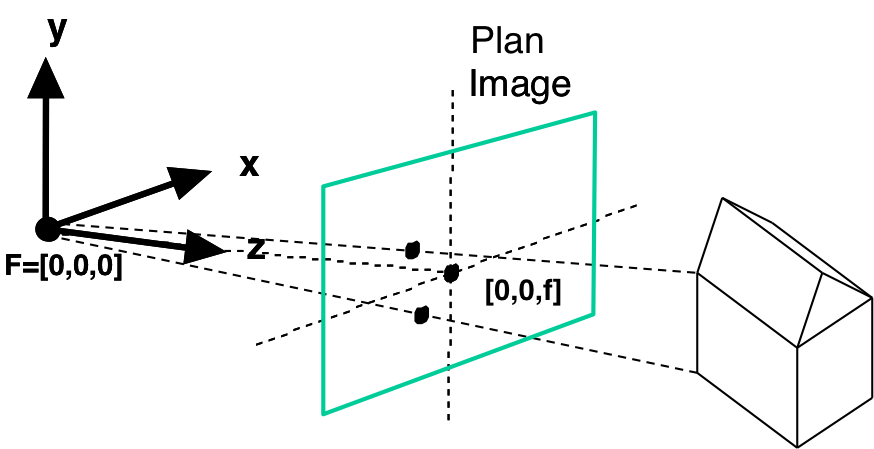
\includegraphics[height=.6\textheight]{figs/persp2.png}
\end{center}
\end{frame}

\begin{frame}{Calcul de la projection}
\begin{eqnarray*}
z' & = & f \\
y'/z' & = & y/z \\
\end{eqnarray*}
\begin{center}
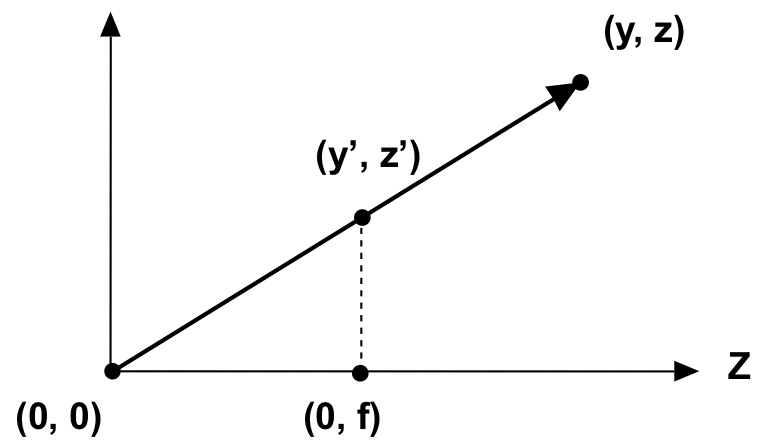
\includegraphics[height=.4\textheight]{figs/persp3.png}
\end{center}
\begin{itemize}
\item Le point $(x,y,z)^t$ se projette sur $\left( (f/z)x,(f/z)y,f \right)^t$
\end{itemize}
\end{frame}

\begin{frame}{Matrice homogène}
\begin{itemize}
\item Projection sur le plan $z=0$ avec le centre de projection placé à $z=-f$

$$
\left(
\begin{array}{cccc}
1 & 0 & 0 & 0 \\
0 & 1 & 0 & 0 \\
0 & 0 & 1 & 0 \\
0 & 0 & \frac{1}{d} & 1
\end{array}
\right)
$$
\item Utilisation de la quatrième coordonnée pour le rétrécissement
\end{itemize}
\end{frame}

\subsection{Autres transformations géométriques}

\begin{frame}{Pyramide de vue (2D)}
\begin{center}
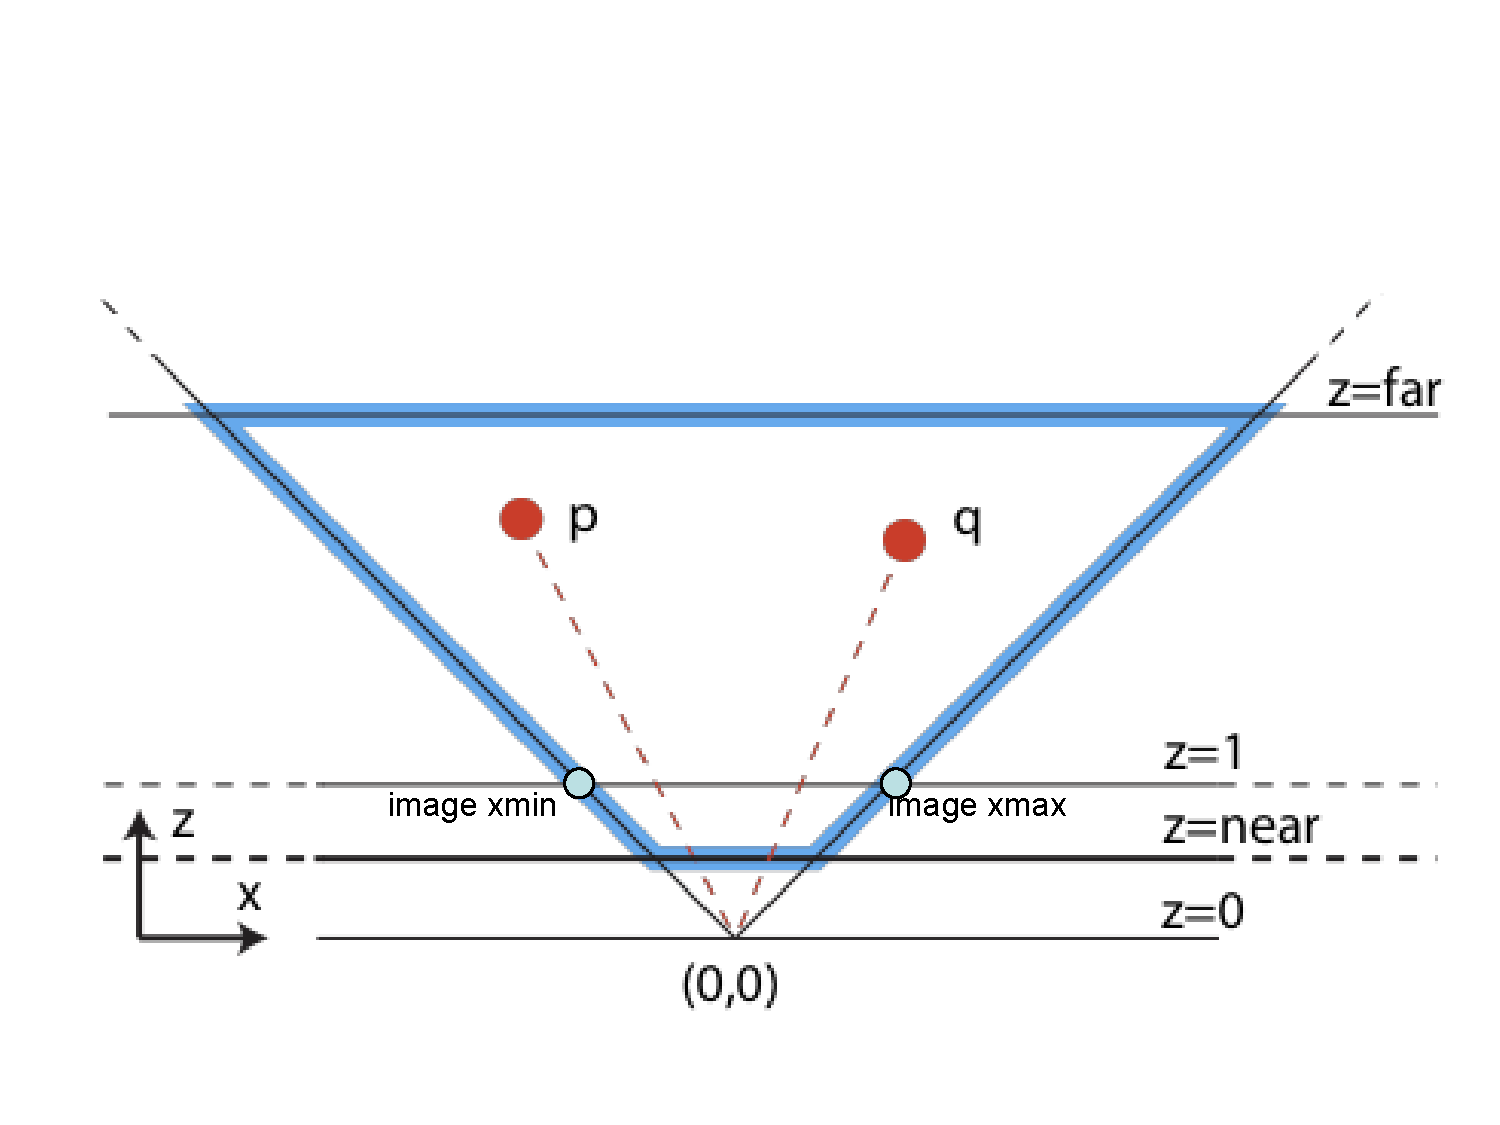
\includegraphics[height=.6\textheight]{figs/frustum2d.pdf}
\end{center}
\end{frame}


\begin{frame}{Clipping}
\begin{columns}
\begin{column}{.6\textwidth}
\begin{itemize}
\item Éliminer les portions des objets qui sont en dehors de la pyramide de vue
\begin{itemize}
\item délimitée par les limites du plan image projeté en 3D et des \textit{near} et \textit{far} plane
\end{itemize}
\item Pourquoi faire ?
\begin{itemize}
\item Ne pas dessiner derrière l'\oe il
\item Limiter la quantité de choses dessinées
\end{itemize}
\item Encore des matrices homogènes !
\end{itemize}
\end{column}
\begin{column}{.39\textwidth}
\begin{center}
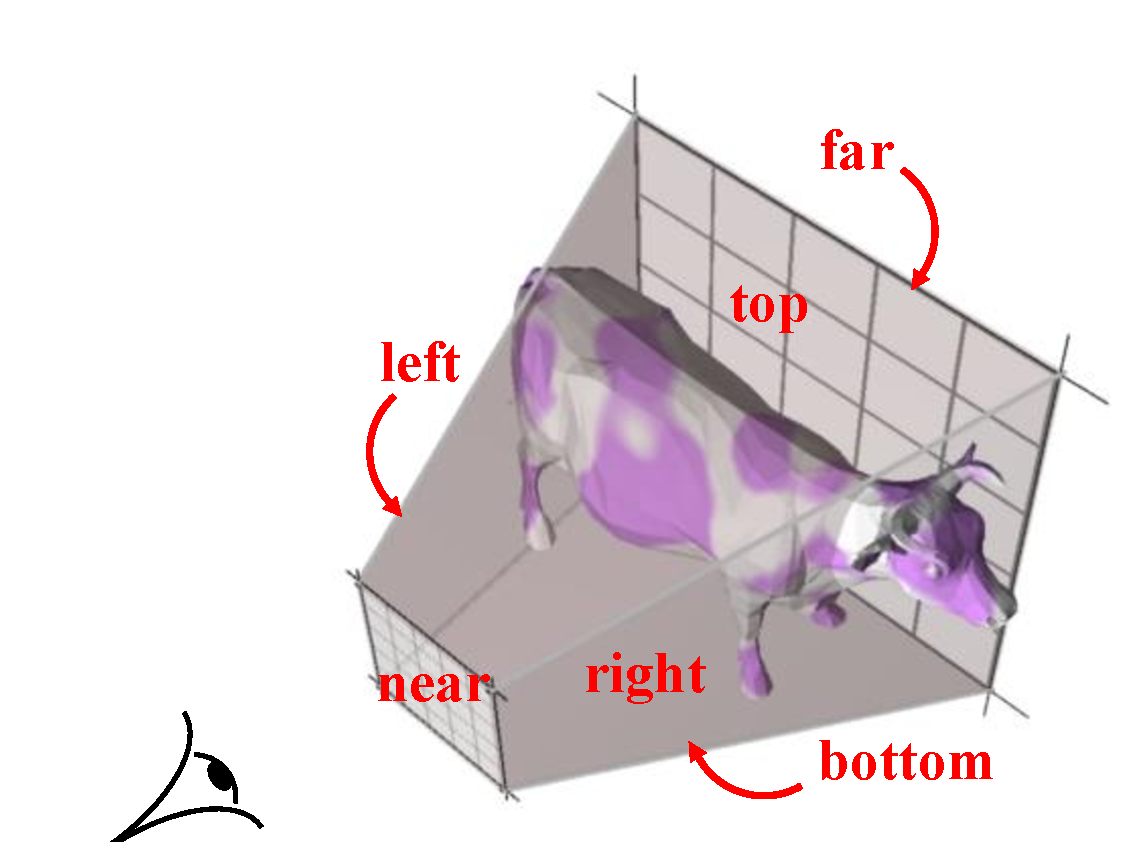
\includegraphics[height=.4\textheight]{figs/frustum3d.pdf}
\end{center}
\end{column}
\end{columns}
\end{frame}

\begin{frame}{Backface culling}
\begin{itemize}
\item Élimination des faces vues par l'arrière
\begin{itemize}
\item valable pour les solides non transparents
\end{itemize}
\item Simple produit scalaire entre la normale à une face et le vecteur reliant l'\oe il à cette face
\end{itemize}
\begin{center}
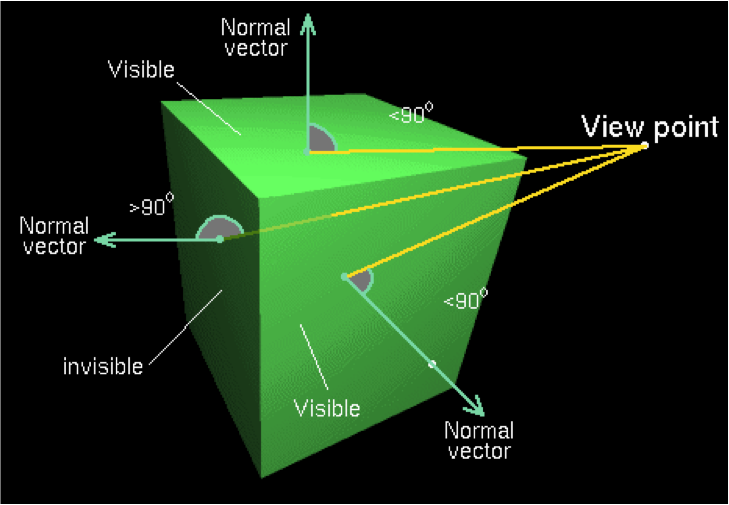
\includegraphics[height=.5\textheight]{figs/bfc.png}
\end{center}
\end{frame}
